\RequirePackage{silence} % :-\
    \WarningFilter{scrreprt}{Usage of package `titlesec'}
    \WarningFilter{scrreprt}{Activating an ugly workaround}
    \WarningFilter{titlesec}{Non standard sectioning command detected}
\documentclass[ twoside,openright,titlepage,numbers=noenddot,%1headlines,
                headinclude,footinclude,cleardoublepage=empty,abstract=on,
                BCOR=5mm,paper=a4,fontsize=11pt
                ]{scrreprt}

% ****************************************************************************************************
% classicthesis-config.tex
% formerly known as loadpackages.sty, classicthesis-ldpkg.sty, and classicthesis-preamble.sty
% Use it at the beginning of your ClassicThesis.tex, or as a LaTeX Preamble
% in your ClassicThesis.{tex,lyx} with % ****************************************************************************************************
% classicthesis-config.tex
% formerly known as loadpackages.sty, classicthesis-ldpkg.sty, and classicthesis-preamble.sty
% Use it at the beginning of your ClassicThesis.tex, or as a LaTeX Preamble
% in your ClassicThesis.{tex,lyx} with % ****************************************************************************************************
% classicthesis-config.tex
% formerly known as loadpackages.sty, classicthesis-ldpkg.sty, and classicthesis-preamble.sty
% Use it at the beginning of your ClassicThesis.tex, or as a LaTeX Preamble
% in your ClassicThesis.{tex,lyx} with \input{classicthesis-config}
% ****************************************************************************************************
% If you like the classicthesis, then I would appreciate a postcard.
% My address can be found in the file ClassicThesis.pdf. A collection
% of the postcards I received so far is available online at
% http://postcards.miede.de
% ****************************************************************************************************


% ****************************************************************************************************
% 0. Set the encoding of your files. UTF-8 is the only sensible encoding nowadays. If you can't read
% äöüßáéçèê∂åëæƒÏ€ then change the encoding setting in your editor, not the line below. If your editor
% does not support utf8 use another editor!
% ****************************************************************************************************
\PassOptionsToPackage{utf8}{inputenc}
  \usepackage{inputenc}

\PassOptionsToPackage{T1}{fontenc} % T2A for cyrillics
  \usepackage{fontenc}


% ****************************************************************************************************
% 1. Configure classicthesis for your needs here, e.g., remove "drafting" below
% in order to deactivate the time-stamp on the pages
% (see ClassicThesis.pdf for more information):
% ****************************************************************************************************
\PassOptionsToPackage{
  drafting=false,    % print version information on the bottom of the pages
  tocaligned=false, % the left column of the toc will be aligned (no indentation)
  dottedtoc=false,  % page numbers in ToC flushed right
  eulerchapternumbers=true, % use AMS Euler for chapter font (otherwise Palatino)
  linedheaders=false,       % chaper headers will have line above and beneath
  floatperchapter=true,     % numbering per chapter for all floats (i.e., Figure 1.1)
  eulermath=false,  % use awesome Euler fonts for mathematical formulae (only with pdfLaTeX)
  beramono=false,    % toggle a nice monospaced font (w/ bold)
  palatino=false,    % deactivate standard font for loading another one, see the last section at the end of this file for suggestions
  style=classicthesis % classicthesis, arsclassica
}{classicthesis}


% ****************************************************************************************************
% 2. Personal data and user ad-hoc commands (insert your own data here)
% ****************************************************************************************************
\newcommand{\myTitle}{Including STDP to eligibility propagation in multi-layer recurrent spiking neural networks\xspace}
\newcommand{\mySubtitle}{Master's Thesis\xspace}
\newcommand{\myDegree}{MSc. Artificial Intelligence\xspace}
\newcommand{\myName}{Werner van der Veen\xspace}
\newcommand{\myProf}{Dr. Herbert Jaeger\xspace}
\newcommand{\myOtherProf}{Dr. Marco Wiering\xspace}
\newcommand{\mySupervisor}{Put name here\xspace}
\newcommand{\myFaculty}{Faculty of Science and Engineering\xspace}
\newcommand{\myDepartment}{Put data here\xspace}
\newcommand{\myUni}{University of Groningen\xspace}
\newcommand{\myLocation}{Groningen, The Netherlands\xspace}
\newcommand{\myTime}{\today\xspace}
\newcommand{\myVersion}{Put version here}

% ********************************************************************
% Setup, finetuning, and useful commands
% ********************************************************************
\providecommand{\mLyX}{L\kern-.1667em\lower.25em\hbox{Y}\kern-.125emX\@}
\newcommand{\ie}{i.\,e.}
\newcommand{\Ie}{I.\,e.}
\newcommand{\eg}{e.\,g.}
\newcommand{\Eg}{E.\,g.}
% ****************************************************************************************************


% ****************************************************************************************************
% 3. Loading some handy packages
% ****************************************************************************************************
% ********************************************************************
% Packages with options that might require adjustments
% ********************************************************************
\PassOptionsToPackage{american}{babel} % change this to your language(s), main language last
% Spanish languages need extra options in order to work with this template
%\PassOptionsToPackage{spanish,es-lcroman}{babel}
\usepackage{babel}

\usepackage{csquotes}
\PassOptionsToPackage{%
  backend=biber,bibencoding=utf8, %instead of bibtex
  % backend=bibtex8,bibencoding=ascii,%
  language=auto,%
  style=authoryear-comp,%
  % style=alphabetic, %
  citestyle=authoryear-comp, % Author 1999, 2010
  bibstyle=authoryear,dashed=false, % dashed: substitute rep. author with ---
  sorting=nyt, % name, year, title
  maxbibnames=3, % default: 3, et al.
  %backref=true,%
  natbib=true % natbib compatibility mode (\citep and \citet still work)
}{biblatex}
    \usepackage{biblatex}

\PassOptionsToPackage{fleqn}{amsmath}       % math environments and more by the AMS
  \usepackage{amsmath}

% ********************************************************************
% General useful packages
% ********************************************************************
\usepackage{graphicx} %
\usepackage{scrhack} % fix warnings when using KOMA with listings package
\usepackage{xspace} % to get the spacing after macros right
\PassOptionsToPackage{printonlyused,smaller}{acronym}
  \usepackage{acronym} % nice macros for handling all acronyms in the thesis
  %\renewcommand{\bflabel}[1]{{#1}\hfill} % fix the list of acronyms --> no longer working
  %\renewcommand*{\acsfont}[1]{\textsc{#1}}
  %\renewcommand*{\aclabelfont}[1]{\acsfont{#1}}
  %\def\bflabel#1{{#1\hfill}}
  \def\bflabel#1{{\acsfont{#1}\hfill}}
  \def\aclabelfont#1{\acsfont{#1}}
% ****************************************************************************************************
%\usepackage{pgfplots} % External TikZ/PGF support (thanks to Andreas Nautsch)
%\usetikzlibrary{external}
%\tikzexternalize[mode=list and make, prefix=ext-tikz/]
% ****************************************************************************************************


% ****************************************************************************************************
% 4. Setup floats: tables, (sub)figures, and captions
% ****************************************************************************************************
\usepackage{tabularx} % better tables
  \setlength{\extrarowheight}{3pt} % increase table row height
\newcommand{\tableheadline}[1]{\multicolumn{1}{l}{\spacedlowsmallcaps{#1}}}
\newcommand{\myfloatalign}{\centering} % to be used with each float for alignment
\usepackage{subfig}
% ****************************************************************************************************


% ****************************************************************************************************
% 5. Setup code listings
% ****************************************************************************************************
\usepackage{listings}
%\lstset{emph={trueIndex,root},emphstyle=\color{BlueViolet}}%\underbar} % for special keywords
\lstset{language=[LaTeX]Tex,%C++,
  morekeywords={PassOptionsToPackage,selectlanguage},
  keywordstyle=\color{RoyalBlue},%\bfseries,
  basicstyle=\small\ttfamily,
  %identifierstyle=\color{NavyBlue},
  commentstyle=\color{Green}\ttfamily,
  stringstyle=\rmfamily,
  numbers=none,%left,%
  numberstyle=\scriptsize,%\tiny
  stepnumber=5,
  numbersep=8pt,
  showstringspaces=false,
  breaklines=true,
  %frameround=ftff,
  %frame=single,
  belowcaptionskip=.75\baselineskip
  %frame=L
}
% ********************************************************************


\usepackage{classicthesis}


% ********************************************************************
% Fine-tune hyperreferences (hyperref should be called last)
% ********************************************************************
\hypersetup{%
  %draft, % hyperref's draft mode, for printing see below
  colorlinks=false, linktocpage=true, pdfstartpage=3, pdfstartview=FitV,%
  % uncomment the following line if you want to have black links (e.g., for printing)
  %colorlinks=false, linktocpage=false, pdfstartpage=3, pdfstartview=FitV, pdfborder={0 0 0},%
  breaklinks=true, pageanchor=true,%
  pdfpagemode=UseNone, %
  % pdfpagemode=UseOutlines,%
  plainpages=false, bookmarksnumbered, bookmarksopen=true, bookmarksopenlevel=1,%
  hypertexnames=true, pdfhighlight=/O,%nesting=true,%frenchlinks,%
  urlcolor=CTurl, linkcolor=CTlink, citecolor=CTcitation, %pagecolor=RoyalBlue,%
  %urlcolor=Black, linkcolor=Black, citecolor=Black, %pagecolor=Black,%
  pdftitle={\myTitle},%
  pdfauthor={\textcopyright\ \myName, \myUni, \myFaculty},%
  pdfsubject={},%
  pdfkeywords={},%
  pdfcreator={pdfLaTeX},%
  pdfproducer={LaTeX with hyperref and classicthesis}%
}

\makeatletter
\@ifpackageloaded{babel}%
  {%
    \addto\extrasamerican{%
      \renewcommand*{\figureautorefname}{Figure}%
      \renewcommand*{\tableautorefname}{Table}%
      \renewcommand*{\partautorefname}{Part}%
      \renewcommand*{\chapterautorefname}{Chapter}%
      \renewcommand*{\sectionautorefname}{Section}%
      \renewcommand*{\subsectionautorefname}{Section}%
      \renewcommand*{\subsubsectionautorefname}{Section}%
    }%
      \providecommand{\subfigureautorefname}{\figureautorefname}%
    }{\relax}
\makeatother

% ****************************************************************************************************
% If you like the classicthesis, then I would appreciate a postcard.
% My address can be found in the file ClassicThesis.pdf. A collection
% of the postcards I received so far is available online at
% http://postcards.miede.de
% ****************************************************************************************************


% ****************************************************************************************************
% 0. Set the encoding of your files. UTF-8 is the only sensible encoding nowadays. If you can't read
% äöüßáéçèê∂åëæƒÏ€ then change the encoding setting in your editor, not the line below. If your editor
% does not support utf8 use another editor!
% ****************************************************************************************************
\PassOptionsToPackage{utf8}{inputenc}
  \usepackage{inputenc}

\PassOptionsToPackage{T1}{fontenc} % T2A for cyrillics
  \usepackage{fontenc}


% ****************************************************************************************************
% 1. Configure classicthesis for your needs here, e.g., remove "drafting" below
% in order to deactivate the time-stamp on the pages
% (see ClassicThesis.pdf for more information):
% ****************************************************************************************************
\PassOptionsToPackage{
  drafting=false,    % print version information on the bottom of the pages
  tocaligned=false, % the left column of the toc will be aligned (no indentation)
  dottedtoc=false,  % page numbers in ToC flushed right
  eulerchapternumbers=true, % use AMS Euler for chapter font (otherwise Palatino)
  linedheaders=false,       % chaper headers will have line above and beneath
  floatperchapter=true,     % numbering per chapter for all floats (i.e., Figure 1.1)
  eulermath=false,  % use awesome Euler fonts for mathematical formulae (only with pdfLaTeX)
  beramono=false,    % toggle a nice monospaced font (w/ bold)
  palatino=false,    % deactivate standard font for loading another one, see the last section at the end of this file for suggestions
  style=classicthesis % classicthesis, arsclassica
}{classicthesis}


% ****************************************************************************************************
% 2. Personal data and user ad-hoc commands (insert your own data here)
% ****************************************************************************************************
\newcommand{\myTitle}{Including STDP to eligibility propagation in multi-layer recurrent spiking neural networks\xspace}
\newcommand{\mySubtitle}{Master's Thesis\xspace}
\newcommand{\myDegree}{MSc. Artificial Intelligence\xspace}
\newcommand{\myName}{Werner van der Veen\xspace}
\newcommand{\myProf}{Dr. Herbert Jaeger\xspace}
\newcommand{\myOtherProf}{Dr. Marco Wiering\xspace}
\newcommand{\mySupervisor}{Put name here\xspace}
\newcommand{\myFaculty}{Faculty of Science and Engineering\xspace}
\newcommand{\myDepartment}{Put data here\xspace}
\newcommand{\myUni}{University of Groningen\xspace}
\newcommand{\myLocation}{Groningen, The Netherlands\xspace}
\newcommand{\myTime}{\today\xspace}
\newcommand{\myVersion}{Put version here}

% ********************************************************************
% Setup, finetuning, and useful commands
% ********************************************************************
\providecommand{\mLyX}{L\kern-.1667em\lower.25em\hbox{Y}\kern-.125emX\@}
\newcommand{\ie}{i.\,e.}
\newcommand{\Ie}{I.\,e.}
\newcommand{\eg}{e.\,g.}
\newcommand{\Eg}{E.\,g.}
% ****************************************************************************************************


% ****************************************************************************************************
% 3. Loading some handy packages
% ****************************************************************************************************
% ********************************************************************
% Packages with options that might require adjustments
% ********************************************************************
\PassOptionsToPackage{american}{babel} % change this to your language(s), main language last
% Spanish languages need extra options in order to work with this template
%\PassOptionsToPackage{spanish,es-lcroman}{babel}
\usepackage{babel}

\usepackage{csquotes}
\PassOptionsToPackage{%
  backend=biber,bibencoding=utf8, %instead of bibtex
  % backend=bibtex8,bibencoding=ascii,%
  language=auto,%
  style=authoryear-comp,%
  % style=alphabetic, %
  citestyle=authoryear-comp, % Author 1999, 2010
  bibstyle=authoryear,dashed=false, % dashed: substitute rep. author with ---
  sorting=nyt, % name, year, title
  maxbibnames=3, % default: 3, et al.
  %backref=true,%
  natbib=true % natbib compatibility mode (\citep and \citet still work)
}{biblatex}
    \usepackage{biblatex}

\PassOptionsToPackage{fleqn}{amsmath}       % math environments and more by the AMS
  \usepackage{amsmath}

% ********************************************************************
% General useful packages
% ********************************************************************
\usepackage{graphicx} %
\usepackage{scrhack} % fix warnings when using KOMA with listings package
\usepackage{xspace} % to get the spacing after macros right
\PassOptionsToPackage{printonlyused,smaller}{acronym}
  \usepackage{acronym} % nice macros for handling all acronyms in the thesis
  %\renewcommand{\bflabel}[1]{{#1}\hfill} % fix the list of acronyms --> no longer working
  %\renewcommand*{\acsfont}[1]{\textsc{#1}}
  %\renewcommand*{\aclabelfont}[1]{\acsfont{#1}}
  %\def\bflabel#1{{#1\hfill}}
  \def\bflabel#1{{\acsfont{#1}\hfill}}
  \def\aclabelfont#1{\acsfont{#1}}
% ****************************************************************************************************
%\usepackage{pgfplots} % External TikZ/PGF support (thanks to Andreas Nautsch)
%\usetikzlibrary{external}
%\tikzexternalize[mode=list and make, prefix=ext-tikz/]
% ****************************************************************************************************


% ****************************************************************************************************
% 4. Setup floats: tables, (sub)figures, and captions
% ****************************************************************************************************
\usepackage{tabularx} % better tables
  \setlength{\extrarowheight}{3pt} % increase table row height
\newcommand{\tableheadline}[1]{\multicolumn{1}{l}{\spacedlowsmallcaps{#1}}}
\newcommand{\myfloatalign}{\centering} % to be used with each float for alignment
\usepackage{subfig}
% ****************************************************************************************************


% ****************************************************************************************************
% 5. Setup code listings
% ****************************************************************************************************
\usepackage{listings}
%\lstset{emph={trueIndex,root},emphstyle=\color{BlueViolet}}%\underbar} % for special keywords
\lstset{language=[LaTeX]Tex,%C++,
  morekeywords={PassOptionsToPackage,selectlanguage},
  keywordstyle=\color{RoyalBlue},%\bfseries,
  basicstyle=\small\ttfamily,
  %identifierstyle=\color{NavyBlue},
  commentstyle=\color{Green}\ttfamily,
  stringstyle=\rmfamily,
  numbers=none,%left,%
  numberstyle=\scriptsize,%\tiny
  stepnumber=5,
  numbersep=8pt,
  showstringspaces=false,
  breaklines=true,
  %frameround=ftff,
  %frame=single,
  belowcaptionskip=.75\baselineskip
  %frame=L
}
% ********************************************************************


\usepackage{classicthesis}


% ********************************************************************
% Fine-tune hyperreferences (hyperref should be called last)
% ********************************************************************
\hypersetup{%
  %draft, % hyperref's draft mode, for printing see below
  colorlinks=false, linktocpage=true, pdfstartpage=3, pdfstartview=FitV,%
  % uncomment the following line if you want to have black links (e.g., for printing)
  %colorlinks=false, linktocpage=false, pdfstartpage=3, pdfstartview=FitV, pdfborder={0 0 0},%
  breaklinks=true, pageanchor=true,%
  pdfpagemode=UseNone, %
  % pdfpagemode=UseOutlines,%
  plainpages=false, bookmarksnumbered, bookmarksopen=true, bookmarksopenlevel=1,%
  hypertexnames=true, pdfhighlight=/O,%nesting=true,%frenchlinks,%
  urlcolor=CTurl, linkcolor=CTlink, citecolor=CTcitation, %pagecolor=RoyalBlue,%
  %urlcolor=Black, linkcolor=Black, citecolor=Black, %pagecolor=Black,%
  pdftitle={\myTitle},%
  pdfauthor={\textcopyright\ \myName, \myUni, \myFaculty},%
  pdfsubject={},%
  pdfkeywords={},%
  pdfcreator={pdfLaTeX},%
  pdfproducer={LaTeX with hyperref and classicthesis}%
}

\makeatletter
\@ifpackageloaded{babel}%
  {%
    \addto\extrasamerican{%
      \renewcommand*{\figureautorefname}{Figure}%
      \renewcommand*{\tableautorefname}{Table}%
      \renewcommand*{\partautorefname}{Part}%
      \renewcommand*{\chapterautorefname}{Chapter}%
      \renewcommand*{\sectionautorefname}{Section}%
      \renewcommand*{\subsectionautorefname}{Section}%
      \renewcommand*{\subsubsectionautorefname}{Section}%
    }%
      \providecommand{\subfigureautorefname}{\figureautorefname}%
    }{\relax}
\makeatother

% ****************************************************************************************************
% If you like the classicthesis, then I would appreciate a postcard.
% My address can be found in the file ClassicThesis.pdf. A collection
% of the postcards I received so far is available online at
% http://postcards.miede.de
% ****************************************************************************************************


% ****************************************************************************************************
% 0. Set the encoding of your files. UTF-8 is the only sensible encoding nowadays. If you can't read
% äöüßáéçèê∂åëæƒÏ€ then change the encoding setting in your editor, not the line below. If your editor
% does not support utf8 use another editor!
% ****************************************************************************************************
\PassOptionsToPackage{utf8}{inputenc}
  \usepackage{inputenc}

\PassOptionsToPackage{T1}{fontenc} % T2A for cyrillics
  \usepackage{fontenc}


% ****************************************************************************************************
% 1. Configure classicthesis for your needs here, e.g., remove "drafting" below
% in order to deactivate the time-stamp on the pages
% (see ClassicThesis.pdf for more information):
% ****************************************************************************************************
\PassOptionsToPackage{
  drafting=false,    % print version information on the bottom of the pages
  tocaligned=false, % the left column of the toc will be aligned (no indentation)
  dottedtoc=false,  % page numbers in ToC flushed right
  eulerchapternumbers=true, % use AMS Euler for chapter font (otherwise Palatino)
  linedheaders=false,       % chaper headers will have line above and beneath
  floatperchapter=true,     % numbering per chapter for all floats (i.e., Figure 1.1)
  eulermath=false,  % use awesome Euler fonts for mathematical formulae (only with pdfLaTeX)
  beramono=false,    % toggle a nice monospaced font (w/ bold)
  palatino=false,    % deactivate standard font for loading another one, see the last section at the end of this file for suggestions
  style=classicthesis % classicthesis, arsclassica
}{classicthesis}


% ****************************************************************************************************
% 2. Personal data and user ad-hoc commands (insert your own data here)
% ****************************************************************************************************
\newcommand{\myTitle}{Including STDP to eligibility propagation in multi-layer recurrent spiking neural networks\xspace}
\newcommand{\mySubtitle}{Master's Thesis\xspace}
\newcommand{\myDegree}{MSc. Artificial Intelligence\xspace}
\newcommand{\myName}{Werner van der Veen\xspace}
\newcommand{\myProf}{Dr. Herbert Jaeger\xspace}
\newcommand{\myOtherProf}{Dr. Marco Wiering\xspace}
\newcommand{\mySupervisor}{Put name here\xspace}
\newcommand{\myFaculty}{Faculty of Science and Engineering\xspace}
\newcommand{\myDepartment}{Put data here\xspace}
\newcommand{\myUni}{University of Groningen\xspace}
\newcommand{\myLocation}{Groningen, The Netherlands\xspace}
\newcommand{\myTime}{\today\xspace}
\newcommand{\myVersion}{Put version here}

% ********************************************************************
% Setup, finetuning, and useful commands
% ********************************************************************
\providecommand{\mLyX}{L\kern-.1667em\lower.25em\hbox{Y}\kern-.125emX\@}
\newcommand{\ie}{i.\,e.}
\newcommand{\Ie}{I.\,e.}
\newcommand{\eg}{e.\,g.}
\newcommand{\Eg}{E.\,g.}
% ****************************************************************************************************


% ****************************************************************************************************
% 3. Loading some handy packages
% ****************************************************************************************************
% ********************************************************************
% Packages with options that might require adjustments
% ********************************************************************
\PassOptionsToPackage{american}{babel} % change this to your language(s), main language last
% Spanish languages need extra options in order to work with this template
%\PassOptionsToPackage{spanish,es-lcroman}{babel}
\usepackage{babel}

\usepackage{csquotes}
\PassOptionsToPackage{%
  backend=biber,bibencoding=utf8, %instead of bibtex
  % backend=bibtex8,bibencoding=ascii,%
  language=auto,%
  style=authoryear-comp,%
  % style=alphabetic, %
  citestyle=authoryear-comp, % Author 1999, 2010
  bibstyle=authoryear,dashed=false, % dashed: substitute rep. author with ---
  sorting=nyt, % name, year, title
  maxbibnames=3, % default: 3, et al.
  %backref=true,%
  natbib=true % natbib compatibility mode (\citep and \citet still work)
}{biblatex}
    \usepackage{biblatex}

\PassOptionsToPackage{fleqn}{amsmath}       % math environments and more by the AMS
  \usepackage{amsmath}

% ********************************************************************
% General useful packages
% ********************************************************************
\usepackage{graphicx} %
\usepackage{scrhack} % fix warnings when using KOMA with listings package
\usepackage{xspace} % to get the spacing after macros right
\PassOptionsToPackage{printonlyused,smaller}{acronym}
  \usepackage{acronym} % nice macros for handling all acronyms in the thesis
  %\renewcommand{\bflabel}[1]{{#1}\hfill} % fix the list of acronyms --> no longer working
  %\renewcommand*{\acsfont}[1]{\textsc{#1}}
  %\renewcommand*{\aclabelfont}[1]{\acsfont{#1}}
  %\def\bflabel#1{{#1\hfill}}
  \def\bflabel#1{{\acsfont{#1}\hfill}}
  \def\aclabelfont#1{\acsfont{#1}}
% ****************************************************************************************************
%\usepackage{pgfplots} % External TikZ/PGF support (thanks to Andreas Nautsch)
%\usetikzlibrary{external}
%\tikzexternalize[mode=list and make, prefix=ext-tikz/]
% ****************************************************************************************************


% ****************************************************************************************************
% 4. Setup floats: tables, (sub)figures, and captions
% ****************************************************************************************************
\usepackage{tabularx} % better tables
  \setlength{\extrarowheight}{3pt} % increase table row height
\newcommand{\tableheadline}[1]{\multicolumn{1}{l}{\spacedlowsmallcaps{#1}}}
\newcommand{\myfloatalign}{\centering} % to be used with each float for alignment
\usepackage{subfig}
% ****************************************************************************************************


% ****************************************************************************************************
% 5. Setup code listings
% ****************************************************************************************************
\usepackage{listings}
%\lstset{emph={trueIndex,root},emphstyle=\color{BlueViolet}}%\underbar} % for special keywords
\lstset{language=[LaTeX]Tex,%C++,
  morekeywords={PassOptionsToPackage,selectlanguage},
  keywordstyle=\color{RoyalBlue},%\bfseries,
  basicstyle=\small\ttfamily,
  %identifierstyle=\color{NavyBlue},
  commentstyle=\color{Green}\ttfamily,
  stringstyle=\rmfamily,
  numbers=none,%left,%
  numberstyle=\scriptsize,%\tiny
  stepnumber=5,
  numbersep=8pt,
  showstringspaces=false,
  breaklines=true,
  %frameround=ftff,
  %frame=single,
  belowcaptionskip=.75\baselineskip
  %frame=L
}
% ********************************************************************


\usepackage{classicthesis}


% ********************************************************************
% Fine-tune hyperreferences (hyperref should be called last)
% ********************************************************************
\hypersetup{%
  %draft, % hyperref's draft mode, for printing see below
  colorlinks=false, linktocpage=true, pdfstartpage=3, pdfstartview=FitV,%
  % uncomment the following line if you want to have black links (e.g., for printing)
  %colorlinks=false, linktocpage=false, pdfstartpage=3, pdfstartview=FitV, pdfborder={0 0 0},%
  breaklinks=true, pageanchor=true,%
  pdfpagemode=UseNone, %
  % pdfpagemode=UseOutlines,%
  plainpages=false, bookmarksnumbered, bookmarksopen=true, bookmarksopenlevel=1,%
  hypertexnames=true, pdfhighlight=/O,%nesting=true,%frenchlinks,%
  urlcolor=CTurl, linkcolor=CTlink, citecolor=CTcitation, %pagecolor=RoyalBlue,%
  %urlcolor=Black, linkcolor=Black, citecolor=Black, %pagecolor=Black,%
  pdftitle={\myTitle},%
  pdfauthor={\textcopyright\ \myName, \myUni, \myFaculty},%
  pdfsubject={},%
  pdfkeywords={},%
  pdfcreator={pdfLaTeX},%
  pdfproducer={LaTeX with hyperref and classicthesis}%
}

\makeatletter
\@ifpackageloaded{babel}%
  {%
    \addto\extrasamerican{%
      \renewcommand*{\figureautorefname}{Figure}%
      \renewcommand*{\tableautorefname}{Table}%
      \renewcommand*{\partautorefname}{Part}%
      \renewcommand*{\chapterautorefname}{Chapter}%
      \renewcommand*{\sectionautorefname}{Section}%
      \renewcommand*{\subsectionautorefname}{Section}%
      \renewcommand*{\subsubsectionautorefname}{Section}%
    }%
      \providecommand{\subfigureautorefname}{\figureautorefname}%
    }{\relax}
\makeatother


\addbibresource{Bibliography.bib}

\usepackage{todonotes} %
\usepackage{siunitx} %
\usepackage{amssymb} %
\usepackage{tcolorbox} %
%\hyphenation{put special hyphenation here}

\begin{document}
\frenchspacing
\raggedbottom
\selectlanguage{american} % american ngerman
%\renewcommand*{\bibname}{new name}
\setbibpreamble{}
\pagenumbering{roman}
\pagestyle{plain}

%********************************************************************
% Frontmatter
%*******************************************************
% %*******************************************************
% Little Dirty Titlepage
%*******************************************************
\thispagestyle{empty}
%\pdfbookmark[1]{Titel}{title}
%*******************************************************
\begin{center}
    \spacedlowsmallcaps{\myName} \\ \medskip

    \begingroup
        \color{CTtitle}\spacedallcaps{\myTitle}
    \endgroup
\end{center}

%*******************************************************
% Titlepage
%*******************************************************
\begin{titlepage}
    %\pdfbookmark[1]{\myTitle}{titlepage}
    % if you want the titlepage to be centered, uncomment and fine-tune the line below (KOMA classes environment)
    \begin{addmargin}[-1cm]{-3cm}
    \begin{center}
        \large

        \hfill

        \vfill

        \begingroup
            \color{CTtitle}\spacedallcaps{\myTitle} \\ \bigskip
        \endgroup

        \spacedlowsmallcaps{\myName}

        \vfill

        % 
\includegraphics[width=6cm]{gfx/TFZsuperellipse_bw} \\ \medskip

        % \mySubtitle \\ \medskip
        % \myDegree \\
        % \myDepartment \\
        \myFaculty \\
        \myUni \\ \bigskip

        \myTime \\ \myVersion

        \vfill

    \end{center}
  \end{addmargin}
\end{titlepage}

\thispagestyle{empty}

\hfill

\vfill

\noindent\myName: \textit{\myTitle,} \mySubtitle, %\myDegree,
\textcopyright\ \myTime

%\bigskip
%
%\noindent\spacedlowsmallcaps{Supervisors}: \\
%\myProf \\
%\myOtherProf \\
%\mySupervisor
%
%\medskip
%
%\noindent\spacedlowsmallcaps{Location}: \\
%\myLocation
%
%\medskip
%
%\noindent\spacedlowsmallcaps{Time Frame}: \\
%\myTime

% \cleardoublepage%*******************************************************
% Dedication
%*******************************************************
\thispagestyle{empty}
\phantomsection
\pdfbookmark[1]{Dedication}{Dedication}

\vspace*{3cm}

\begin{center}
    \emph{Ohana} means family. \\
    Family means nobody gets left behind, or forgotten. \\ \medskip
    --- Lilo \& Stitch
\end{center}

\medskip

\begin{center}
    Dedicated to the loving memory of Rudolf Miede. \\ \smallskip
    1939\,--\,2005
\end{center}


% \cleardoublepage\include{FrontBackmatter/Foreword}

% \cleardoublepage%*******************************************************
% Abstract
%*******************************************************
%\renewcommand{\abstractname}{Abstract}
\pdfbookmark[1]{Abstract}{Abstract}
% \addcontentsline{toc}{chapter}{\tocEntry{Abstract}}
\begingroup
\let\clearpage\relax
\let\cleardoublepage\relax
\let\cleardoublepage\relax

\chapter*{Abstract}
Spiking neural networks (SNNs) in neuromorphic systems are more energy efficient compared to deep learning--based methods, but there is no clear competitive learning algorithm for training such SNNs.
Eligibility propagation (e-prop) offers an efficient and biologically plausible way to train competitive recurrent SNNs in low-power neuromorphic hardware.
In this report, previous performance of e-prop on a speech classification task is reproduced, and the effects of including STDP-like behavior are analyzed.
Including STDP to the ALIF neuron model improves the classification performance, but this is not the case for the Izhikevich e-prop neuron.
Finally, it was found that e-prop implemented in a single-layer recurrent SNN consistently outperforms a multi-layer variant.

\endgroup

\vfill

% \cleardoublepage%*******************************************************
% Publications
%*******************************************************
\pdfbookmark[1]{Publications}{publications}
\chapter*{Publications}\graffito{This is just an early --~and currently ugly~-- test!}
This might come in handy for PhD theses: some ideas and figures have appeared previously in the following publications:

%\noindent Put your publications from the thesis here. The packages \texttt{multibib} or \texttt{bibtopic} etc. can be used to handle multiple different bibliographies in your document.

\begin{refsection}[ownpubs]
    \small
    \nocite{*} % is local to to the enclosing refsection
    \printbibliography[heading=none]
\end{refsection}

\emph{Attention}: This requires a separate run of \texttt{bibtex} for your \texttt{refsection}, \eg, \texttt{ClassicThesis1-blx} for this file. You might also use \texttt{biber} as the backend for \texttt{biblatex}. See also \url{http://tex.stackexchange.com/questions/128196/problem-with-refsection}.

% \cleardoublepage%*******************************************************
% Acknowledgments
%*******************************************************
\pdfbookmark[1]{Acknowledgments}{acknowledgments}

\begin{flushright}{\slshape
    We have seen that computer programming is an art, \\
    because it applies accumulated knowledge to the world, \\
    because it requires skill and ingenuity, and especially \\
    because it produces objects of beauty.} \\ \medskip
    --- \defcitealias{knuth:1974}{Donald E. Knuth}\citetalias{knuth:1974} \citep{knuth:1974}
\end{flushright}



\bigskip

\begingroup
\let\clearpage\relax
\let\cleardoublepage\relax
\let\cleardoublepage\relax
\chapter*{Acknowledgments}
Put your acknowledgments here.

Many thanks to everybody who already sent me a postcard!

Regarding the typography and other help, many thanks go to Marco
Kuhlmann, Philipp Lehman, Lothar Schlesier, Jim Young, Lorenzo
Pantieri and Enrico Gregorio\footnote{Members of GuIT (Gruppo
Italiano Utilizzatori di \TeX\ e \LaTeX )}, J\"org Sommer,
Joachim K\"ostler, Daniel Gottschlag, Denis Aydin, Paride
Legovini, Steffen Prochnow, Nicolas Repp, Hinrich Harms,
Roland Winkler, Jörg Weber, Henri Menke, Claus Lahiri,
Clemens Niederberger, Stefano Bragaglia, Jörn Hees,
Scott Lowe, Dave Howcroft, Jos\'e M. Alcaide, David Carlisle,
Ulrike Fischer, Hugues de Lassus, Csaba Hajdu, Dave Howcroft, 
and the whole \LaTeX-community for support, ideas and
some great software.

\bigskip

\noindent\emph{Regarding \mLyX}: The \mLyX\ port was intially done by
\emph{Nicholas Mariette} in March 2009 and continued by
\emph{Ivo Pletikosi\'c} in 2011. Thank you very much for your
work and for the contributions to the original style.


\endgroup

\cleardoublepage%*******************************************************
% Table of Contents
%*******************************************************
\pagestyle{scrheadings}
%\phantomsection
\pdfbookmark[1]{\contentsname}{tableofcontents}
\setcounter{tocdepth}{2} % <-- 2 includes up to subsections in the ToC
\setcounter{secnumdepth}{3} % <-- 3 numbers up to subsubsections
\manualmark
\markboth{\spacedlowsmallcaps{\contentsname}}{\spacedlowsmallcaps{\contentsname}}
\tableofcontents
\automark[section]{chapter}
\renewcommand{\chaptermark}[1]{\markboth{\spacedlowsmallcaps{#1}}{\spacedlowsmallcaps{#1}}}
\renewcommand{\sectionmark}[1]{\markright{\textsc{\thesection}\enspace\spacedlowsmallcaps{#1}}}
%*******************************************************
% List of Figures and of the Tables
%*******************************************************
\clearpage
% \pagestyle{empty} % Uncomment this line if your lists should not have any headlines with section name and page number
\begingroup
    \let\clearpage\relax
    \let\cleardoublepage\relax
    %*******************************************************
    % List of Figures
    %*******************************************************
    %\phantomsection
    %\addcontentsline{toc}{chapter}{\listfigurename}
    \pdfbookmark[1]{\listfigurename}{lof}
    \listoffigures

    \vspace{8ex}

    %*******************************************************
    % List of Tables
    %*******************************************************
    %\phantomsection
    %\addcontentsline{toc}{chapter}{\listtablename}
    \pdfbookmark[1]{\listtablename}{lot}
    \listoftables

    \vspace{8ex}
    % \newpage

    %*******************************************************
    % List of Listings
    %*******************************************************
    %\phantomsection
    %\addcontentsline{toc}{chapter}{\lstlistlistingname}
    \pdfbookmark[1]{\lstlistlistingname}{lol}
    % \lstlistoflistings

    \vspace{8ex}

    %*******************************************************
    % Acronyms
    %*******************************************************
    %\phantomsection
    % \pdfbookmark[1]{Acronyms}{acronyms}
    % \markboth{\spacedlowsmallcaps{Acronyms}}{\spacedlowsmallcaps{Acronyms}}
    % \chapter*{Acronyms}
    % \begin{acronym}[UMLX]
    %     \acro{ANN}{Artificial neural network}
    % \end{acronym}

\endgroup


%********************************************************************
% Mainmatter
%*******************************************************
\cleardoublepage
\pagestyle{scrheadings}
\pagenumbering{arabic}
\cleardoublepage


%************************************************
\chapter{Introduction}\label{ch:introduction}
%************************************************

The human brain is one of the most complex systems in the universe.
Its approximately 86 billion neurons \citep{azevedo2009equal} and 100--500 trillion synapses \citep{drachman2005we} are capable of abstract reasoning, pattern recognition, memorization, and sensory experience---while consuming only about \SI{20}{\watt} of power \citep{sokoloff1960metabolism,drubach2000brain}.

An early goal of artificial intelligence has been to construct systems that exhibit similar intelligent traits \citep{turing1948intelligent}.
One of the proposed methods was to emulate the network of biological neurons in the human brain using simple units called perceptrons \citep{rosenblatt1958perceptron}.
These perceptrons were inspired by Hebbian learning \citep{hebb1949organization}, which was a new (and later corroborated) theory on biological learning.
This proved to be more difficult than initially hoped, partly due to ostensibly insurmountable problems such as the inability of perceptrons to learn linearly inseparable tasks \citep{minsky2017perceptrons}.
As a consequence, excitement waned, funding dried up \citep{crevier1993ai}, and the field began focusing on more practical applications, such as expert systems and symbolic reasoning \citep{haugeland1985artificial}.
After the popularization in the 1980s of trainable Hopfield networks \citep{hopfield1982neural} and backpropagation \citep{rumelhart1986learning}, which enabled learning linearly inseparable tasks, artificial neural networks (ANNs) and the connectionist approach were embraced with a new appreciation.

These ANNs are networks of small computational units that can be trained to perform specific pattern recognition tasks.
Backpropagation has proven to work well in training ANNs with multiple layers, most popularly in the field of deep learning (DL), which has become a dominant field in artificial intelligence.
This popularity is partly due to exponentially increasing computing power and data storage capabilities, as well as the rise of the Internet, which has also provided ample training data.
Some variations on ANNs have shown to improve learning performance, such as using convolutional (CNN) and recurrent (RNN) neural networks, both of which are, like the perceptron, inspired by the architecture of the human brain \citep{hubel1968receptive, fukushima1982neocognitron,lecun1995convolutional,lukovsevivcius2009reservoir}.
These types of networks approach or exceed human level performance in some areas \citep{schmidhuber2015deep}.

\paragraph{Energy limits}
However, DL-based methods are starting to show diminishing returns; training some state-of-the-art models can require so much data and computing power that only a small number of organizations has the resources to train and deploy them.
The computational processes of self-driving cars, for example, consume on the order of a thousand watts.
One of the current top submissions of the ``Labeled Faces in the Wild'' face verification task is a deep ANN by Paravision that was trained using a dataset of 10 million face images of 100 thousand individuals\footnote{See \texttt{http://vis-www.cs.umass.edu/lfw/results.html\#everai}. Last accessed January 2021.}.
Beside very large datasets, deep ANNs also require a significant amount of power to train.
For instance, ResNet \citep{he2016deep} has been trained for 3 weeks on a 8-GPU server consuming about 1 GWh.
A more extreme case is the 11-billion parameter version of Google's T5 model \citep{raffel2019exploring}, which is estimated to cost more than \$1.3 million per training run \citep{sharir2020cost}.
This high power consumption precludes computations in mobile low-power or small-scale devices, which now require at least a connection to a cloud computing server.

The energy consumption of DL contrasts strongly with that of the human brain, which can learn patterns using far less energy and data.
This is because despite the biologically inspired foundation, deep ANNs are fundamentally different from the brain, which is an inherently time-dependent dynamical system \citep{sacramento2018dendritic, wozniak2020deep} that relies on biophysical processes, recurrence, and feedback of its physical substrate for computation \citep{sterling2015principles,bhalla2014molecular}.
Deep ANNs are implemented on von Neumann architectures \citep{von1993first}, \ie, a system with a central processing unit (CPU) and separate memory, which are significantly different from the working model of the brain \citep{schuman2017survey}.

One reason for the inefficiency of deep ANNs is that their implementations suffer from the von Neumann bottleneck \citep{zenke2021brain}, which involves a limited throughput between the CPU and memory---a data operation cannot physically co-occur with fetching instructions to process that data because they share the same communication system.
Parallelization on GPUs has alleviated this bottleneck to some extent, but the human brain is more efficient as it is embedded in a physical substrate whose neurons operate and communicate fully in parallel \citep{a2017parallel} using sparsely occurring \emph{spikes} \citep{bear2020neuroscience}, and where no explicit data processing instructions exist.
A spike can be represented as a binary value which causes the synapse to increase the membrane potential in the efferent neuron to change by a fixed value \citep{bear2020neuroscience}.
Connections in ANNs are represented abstractly by large weight matrices, which are all multiplied with neuron activation values at every propagation cycle.
In the brain, a synapse spikes sparsely and thereby saves energy while conveniently including an informative temporal component.

A second reason is that backpropagation requires two passes over the ANN: the first to compute the network output given an input, and the second to propagate the output error back into the network to move the weights between neurons in the direction of the negative gradient.
Backpropagation in RNNs is often performed by unrolling the network in a feedforward ANN in a process called backpropagation through time (BPTT).
The human brain, in contrast, is unlikely to use backpropagation, BPTT, or gradients of the output error \citep{lillicrap2019backpropagation}.

\paragraph{Spiking neural networks}
Spiking neural networks (SNNs) \citep{maass1997networks,gerstner2002spiking} are another step towards biological plausibility of connectionist models.
The concept dates back to the 1980s \citep{hopfield1982neural}; nevertheless, they are sometimes considered as the third generation of ANNs \citep{maass1997networks}.
SNNs use neurons that do not relay continuous activation values at every propagation cycle, but spike once when they reach a threshold value.
SNNs are competitive to ANNs in terms of accuracy and computational power, as well in their ability to display precise spike timings \citep{lobo2020spiking}.
Their sparse firing regimes also offer improved interpretability of their behavior as compared to traditional ANNs \citep{soltic2010knowledge}, which is desired in areas such as medicine or aviation.

However, SNNs have not been as popular as ANNs.
One reason for this is that spike-based activation is not differentiable.
As a consequence, backpropagation cannot be directly used to move in the negative direction of the error gradient, although some attempts have been made to bridge this divide \citep{bohte2002error,hong2010cooperative,xu2013supervised,ourdighi2016efficient,lee2016training,sacramento2018dendritic,bellec2019biologically,whittington2019theories} and to make backpropagation more biologically plausible.

Similarly, it has been demonstrated that approximations of BPTT can be applied to recurrent SNNs (RSNNs) \citep{huh2017gradient,bellec2018long}.
Other RSNN training methods rely on control theory to train a chaotic reservoir of neurons \citep{thalmeier2016learning,gilra2017predicting}.
Information locality can be preserved in some of these methods \citep{alemi2018learning}, \ie, a neuron or synapse can only access information of itself, or the communication of synapses or neurons (resp.) with which it is directly connected.
The FORCE training method \citep{nicola2017supervised}, in contrast, can also train RSNNs but is nonlocal and therefore not suited for biologically plausible implementations.
This body of research led to increased understanding of training SNNs and how to obtain better learning performances.
For instance, both single- and multi-layer SNNs have shown good performance in visual processing \citep{escobar2009action,kheradpisheh2018stdp,liu2017fast} and speech recognition \citep{tavanaei2017bio,dong2018unsupervised}.
However, none of these algorithms are biologically plausible.
While DL was rapidly becoming popular during the 2010s, there was no clear learning algorithm for SNNs that could compete with ANNs.
A second reason for the relative unpopularity of SNNs is that they are generally emulated in von Neumann architectures, undermining their energy efficiency advantages.

\paragraph{Neuromorphic computing}  % Gives importance to local & online
SNN learning algorithms are particularly useful in the upcoming field of neuromorphic computing (NC) \citep{mitra2008real}, in which analog very-large-scale integration (VLSI) systems are used to implement neural systems.
On the surface, it can be understood as running neural networks not abstracted in a digital system, but physically embedded in a dedicated analog medium.
A central advantage of NC is energy efficiency \citep{hasler1990vlsi,lee1990parallel,tarassenko1990real}.
This energy efficiency, combined with NC's massive parallelism \citep{monroe2014neuromorphic}, makes VLSIs particularly relevant for implementing SNNs.

Like SNNs, neuromorphic systems typically use sparse, event-based communication between devices such as memristors \citep{maan2016survey} and physically colocalized memory and computation \citep{sterling2015principles,neftci2018data}.
Although colocalized memory and computation has also been implemented in von Neumann machines, such as Google's TPU\footnote{See \texttt{https://cloud.google.com/tpu/docs/tpus}. Last accessed January 2021}, Graphcore's IPU\footnote{See \texttt{https://www.graphcore.ai/products/ipu}. Last accessed January 2021}, or Cerebras' CS-1\footnote{See \texttt{https://cerebras.net/product/\#chip}. Last accessed January 2021}, neuromorphic systems are more efficient for running ANNs \citep{merolla2014million,rajendran2019low}.
The energy consumption of CMOS artificial neurons is several orders of magnitude lower than that of neurons in an ANN, and even 2--3 times lower than the energy consumption of biological neurons \citep{elbez2020progressive}.
Neuromorphic systems are also more tolerant to device variation \citep{yu2013low}.

Because of this massive parallelism, high energy efficiency, good error tolerance, and good ability to implement cognitive functions, neuromorphic systems are attracting strong interest.
In particular, SNNs emerged as an ideal biologically inspired NC paradigm for realizing energy-efficient on-chip intelligence hardware \citep{merolla2014million,davies2018loihi}, suitable for running fast and complex SNNs on low-power devices.
For instance, a competitive image classification performance was reached with a 6-order of magnitude speedup in a leaky integrate-and-fire (LIF) SNN in field-programmable gate arrays, compared to digital simulations \citep{zhang2020low}.

\paragraph{Biological learning}
To run an SNN on neuromorphic hardware, a \emph{local} and \emph{online} algorithm is needed.
The precondition of locality refers to the idea that a neuron or synapse can only access information or communication with which it is physically connected.
For instance, the inner state of a neuron can only be influenced by itself, or by the spikes it receives from afferent neurons.
Similarly, a synapse can only spike or change its weight based on signals from the afferent and efferent neuron.
This is a direct consequence of the colocalization of processing and memory.
The precondition of being online can be regarded as temporal locality---neurons and synapses can only access information that physically exists at the same point in time.
They cannot access future information, nor past information if it was not explicitly retained.

The brain also adheres to these two constraints.
Some of the more common learning rules in ANNs are based on a form of Hebbian learning, which is a major factor in biological learning and memory consolidation \citep{schuman2017survey}.
Classical Hebbian learning is often summarized by ``cells that fire together, wire together'', if there is a causal relationship between these cells, such as a postsynaptic potential on a connecting synapse.
Direct application of Hebbian learning in a spiking neural network will generally lead to a positive feedback loop, because ``wiring cells together'', or increasing the synaptic strength, will in turn increase the likelihood that they also fire together \citep{zenke2017temporal}.
Furthermore, classical Hebbian learning describes no way for a synapse to weaken.

Spike-timing-dependent plasticity (STDP) \citep{abbott2000synaptic,caporale2008spike} is a type of Hebbian learning that incorporates temporal causality on a synapse from neuron $A$ to neuron $B$: if $B$ spikes right after neuron $A$, then the synapse is strengthened, but if $B$ spikes right before $A$, it is weakened.
% However, this too leads to runaway activity through the same positive feedback loop.
It is widely known that STDP is a fundamental learning principle in the human brain \citep{kandel2000principles,caporale2008spike}, including perceptual systems in the sensory cortex \citep{huang2014associative}.
STDP by itself can be used as an unsupervised learning algorithm or to forming associations in classical conditioning \citep{diehl2015unsupervised,kim2018demonstration}.
Furthermore, it has been demonstrated to form associations between memory traces in SNNs, which are crucial for cognitive brain function \citep{pokorny2020stdp}.
To allow supervised learning, or operant conditioning, a learning signal is required to influence the direction of the synapse weight change: a positive learning signal will reinforce the association (long-term potentiation), and a negative learning signal weakens it (long term depression) \citep{lobov2020spatial}.
STDP with a learning signal is known as reward-modulated STDP (R-STDP) \citep{legenstein2008learning} in the field of SNNs and three-factor Hebbian learning in neuroscience \citep{fremaux2016neuromodulated}.
Three-factor Hebbian learning has been demonstrated to outperform its classical two-factor counterpart in a localization-and-retrieval task \citep{porr2007learning}.
A possible reason for this performance difference is that modulatory signals ``may provide the attentional and motivational significance for long-term storage of a memory in the brain'' and stabilize classical Hebbian learning \citep{bailey2000heterosynaptic}.


Neurotransmitters are used to modulate the learning signal in the brain.
Dopamine, for instance, which has a central behavioral and functional role in the primary motor cortex \citep{barnes2005activity,dang2006disrupted}, has been shown to modulate synapses through dendritic spine enlargement during a very narrow time window \citep{dang2006disrupted}.
It is behaviorally related to novelty and reward prediction \citep{li2003dopamine,schultz2007behavioral} by gating neuroplasticity of corticostriatal \citep{reynolds2001cellular,reynolds2002dopamine} and ventral tegmental (VTA) synapses \citep{bao2001cortical}.
In the VTA, dopaminergic neurons respond to learning signals in a highly localized manner that is specific for local populations of neurons \citep{engelhard2019specialized}.
This is also the case in other areas of the midbrain \citep{roeper2013dissecting}.
Acetylcholine is another example of a neuromodulator that gates synaptic plasticity in the cortex and enables state-dependent learning, in which memories are recalled better if the sensory context is similar to that during the memory encoding \citep{shulz2000neuronal}.

However, R-STDP by itself does not solve the credit assignment problem, which relates to neuromodulation of synapses after a learning signal is presented with some delay.
In that case, when the learning signal is presented, the neurons have long spiked, and it is not clear which synapses elicited the behavior that is rewarded or punished.
Recent research suggests that the brain uses \emph{eligibility traces} \citep{izhikevich2007solving,florian2007reinforcement} to solve the credit assignment problem \citep{stolyarova2018solving,gerstner2018eligibility}.
In particular, the synaptic CaMKII protein complex is activated during the induction of long-term potentiation (LTP) of biological synapses if the presynaptic neuron spikes shortly before a postsynaptic neuron \citep{sanhueza2013camkii}.
This LTP is maintained over behavioral time spans, and gradually fades.
When followed by a learning signal in the form of a neurotransmitter, synaptic plasticity is induced \citep{yagishita2014critical,cassenaer2012conditional,gerstner2018eligibility}.

Over the past decade, eligibility traces have been researched in the context of a wide range of topics, such as biological learning, spiking neural networks, and neuromorphic computing.
Synaptic plasticity was demonstrated using eligibility traces in deep feedforward SNNs \citep{zenke2018superspike,neftci2017event,kaiser2020synaptic} and could be implemented in feedforward VLSIs.
In \citet{zenke2018superspike} it is asserted that these methods are also applicable for RSNNs.
Eligibility traces have also been shown to solve difficult credit assignment problems in SNNs using R-STDP \citep{legenstein2008learning, bellec2020solution} and in RNNs \citep{he2015distinct}, and have a predictable learning effect \citep{legenstein2008learning}.
R-STDP in SNNs has been used to solve a number of tasks, including training a stable lane keeping controller \citep{bing2020indirect}, but can suffer from catastrophic forgetting and lack of policy evaluation in mapless navigation \citep{bing2018end}.
More recently, \citet{demirag2021pcm} have shown that phase change memory (PCM) devices allow eligibility traces to linger over behavioral timescales in CMOS/memristive architectures.

\paragraph{Eligibility propagation}
Eligibility propagation (e-prop) \citep{bellec2020solution} is a local and online learning algorithm for RSNNs that can be mathematically derived as an approximation to BPTT (see also Section \ref{sec:derivefromBPTT}).
The main aspect that distinguishes e-prop from other eligibility trace--based algorithms is that the particular computation of the eligibility trace depends on multiple hidden states of a neuron.
The property that a neuron can have multiple hidden states means that there are many types of neuron models that can be used in e-prop.

In e-prop, the learning signal is a local variation on random broadcast alignment, which propagates the error directly back onto the neurons with a random weight, resembling the function of a neuromodulator in the brain.
This has been suggested to provide a diversity of feature detectors for task-relevant network inputs \citep{bellec2020solution}.
Broadcast alignment can perform as effectively as backpropagation in some tasks in feedforward ANNs \citep{lillicrap2016random,nokland2016direct} and multi-layer SNNs \citep{samadi2017deep,clopath2010connectivity}, but performs poorly in deep feedforward ANNs for complex image classification tasks \citep{bartunov2018assessing}.

The local and online properties of e-prop make it a biologically plausible learning algorithm that can be implemented on VLSIs.
E-prop has been demonstrated to work for a large variety of tasks, including classifying phones (\ie, speech sounds), for which it performs competitively with LSTMs \citep{graves2013speech}, a popular RNN architecture that uses BPTT.

The fading eligibility trace in e-prop is similar to STDP in that the weight change is smaller if there is a longer delay between a presynaptic and postsynaptic spike.
However, e-prop is essentially independent of STDP, because it does not explicitly relate the order of the pre- and postsynaptic spike to the synaptic weight update.
However, in \citet{bellec2020solution} e-prop is remarked to start showing STDP-like properties if the synaptic delay of a spike is prolonged.

So far, only the LIF and adaptive LIF (ALIF) neuron models have been used in e-prop, which do not show STDP-like properties by default.
In \citet{traub2020learning}, a functional modification was made to the LIF model such that STDP can occur.
In particular, STDP occurs when the neuron model provides a negated gradient signal in the case when a presynaptic signal arrives too late.
This resembles the biological phenomenon of error-related negativity (ERN) \citep{nieuwenhuis2001error}, which is a negative brain response that immediately follows an erroneous behavioral response and peaks after 80--150 ms with an amplitude that depends on the intent and motivation of a person.
\citet{traub2020learning} also showed this effect for the Izhikevich neuron \citep{izhikevich2003simple}.
However, these STDP-modified neurons were shown only in a single-synapse demo to illustrate the STDP properties, not in a full learning task.

\paragraph{Multi-layer RSNNs}
The human neocortex, which is responsible for processing sensory information, controlling motor output, and mediating higher-order cognitive functions, is organized into six recurrent layers of spiking neurons \citep{greig2013molecular}.

The discovery of backpropagation allowed gradient descent--based training of multi-layer ANNs, which significantly increased their performance.
Although it is unlikely to use backpropagation, the human brain is hierarchically structured such that early layers process simple information and deep layers process more abstract information.
Similarly, multi-layer CNNs also show higher levels of abstraction in deeper layers of the network.
For instance, early convolutional filters identify lines and edges, while deeper filters identify more complex shapes.
In RNNs, stacking recurrent layers results in a similar abstraction---but it is temporal instead of spatial \citep{hermans2013training,gallicchio2017deep}.
Deeper RNN layers exhibit slower time dynamics and longer memory spans than shallow layers \citep{gallicchio2018short}, suggesting that they ignore small variations in the input signal and integrate larger temporal patterns.
It is unclear if these findings extrapolate to RSNNs.

\paragraph{This research}
In this report, the performance of e-prop in \citet{bellec2020solution} is reproduced.
Whereas e-prop was implemented using automatic differentiation in that research, in this report it is done explicitly, using the e-prop learning equations, thereby verifying that they are derived correctly.
Furthermore, the two new STDP neuron models that were suggested in \citet{traub2020learning} are experimentally verified for the first time in the TIMIT phone classification task.
One of these models, the STDP-LIF, will be modified to a new adaptive version called STDP-ALIF, thereby linking the ALIF and STDP-LIF neurons models described in \citet{bellec2020solution} and \citet{traub2020learning}, respectively.
In this research, the first question to be answered is whether inclusion of STDP-like behavior in ALIF neurons or Izhikevich neurons can lead to a more accurate and efficient phone classification.
The second research question is whether stacking multiple RSNN layers in an e-prop model will improve the classification accuracy and efficiency.

Chapter \ref{ch:relatedwork} describes the basic version of the e-prop framework.
Chapter \ref{ch:method} describes the method used to implement the TIMIT learning task and modify the e-prop algorithm to a multi-layer framework with different neuron models.
The results are presented and discussed in Chapter \ref{ch:discussion}.
Finally, Chapter \ref{ch:conclusion} concludes this report.

%************************************************
\chapter{Method}\label{ch:method}
%************************************************
\section{Data Preprocessing}

	\subsection{The TIMIT speech corpus}
		TIMIT is a speech corpus that contains phonemically transcribed speech~\citep{garofolo1993darpa}, comprising 6300 sentences, 10 spoken by each of the 630 speakers.
		To include a broad range of dialects all speakers lived in 8 different geographical regions in the United States (as categorized in \cite{labov2008atlas}) during their childhood years.
		Table~\ref{tab:dialects} breaks down the precise composition of the dialect distribution.

		\begin{table}[ht]
		    \myfloatalign
		    \begin{tabularx}{\textwidth}{lrrr} \toprule
		        \tableheadline{Dialect region} & \tableheadline{\#Male}
		        & \tableheadline{\#Female} & \tableheadline{Total} \\ \midrule
		        % Phantoms take care of right-alignment (works iff monospaced digits)
		        1 (New England)   & 31 (63\%) & 18 (27\%) &  49  \phantom{0}(8\%)  \\
		        2 (Northern)      & 71 (70\%) & 31 (30\%) & 102 (16\%) \\
		        3 (North Midland) & 79 (67\%) & 23 (23\%) & 102 (16\%) \\
		        4 (South Midland) & 69 (69\%) & 31 (31\%) & 100 (16\%) \\
		        5 (Southern)      & 62 (63\%) & 36 (37\%) &  98 (16\%) \\
		        6 (New York City) & 30 (65\%) & 16 (35\%) &  46  \phantom{0}(7\%)  \\
		        7 (Western)       & 74 (74\%) & 26 (26\%) & 100 (16\%) \\
		        8                 & 22 (67\%) & 11 (33\%) &  33  \phantom{0}(5\%)  \\
		        \midrule
		        All  & 438 (70\%) & 192 (30\%) & 630 (100\%) \\
		        \bottomrule
		    \end{tabularx}
		    \caption[TIMIT Dialect Regions]{Distibution of speakers' dialect regions and sexes. Speakers of the innominate dialect region 8 relocated often during their childhood.}  \label{tab:dialects}
		\end{table}

		The sentence text can be categorized into 2 \emph{dialect} sentences, 450 \emph{phonetically compact} sentences, and 1890 \emph{phonetically diverse} sentences.

		The dialect sentences, which are spoken by all speakers, are designed to expose the dialectical variants of the speakers.
		The phonetically compact sentences are designed to include many pairs of phones.
		The phonetically diverse sentences are taken from the Brown Corpus~\citep{kucera1967computational} and the Playwrights Dialog~\citep{hultzsch1964tables} in order to maximize the number of allophones (\ie, different phones used to pronounce the same phoneme).
		Table~\ref{tab:types} lists an overview of the distribution of the number of speakers per sentence type.

		\begin{table}[ht]
		    \myfloatalign
		    \begin{tabularx}{\textwidth}{lrrrr} \toprule
		        \tableheadline{Sentence type} & \tableheadline{\#Sentences}
		        & \tableheadline{\#Speakers} & \tableheadline{Total} \\ \midrule
		        % Phantoms take care of right-alignment (works iff monospaced digits)
		        Dialect & 2    & 630 & 1260\\
		        Compact & 450  & 7   & 3150 \\
		        Diverse & 1890 & 1   & 1890 \\
		        \midrule
		        Total   & 2342 &     & 6300 \\
		        \bottomrule
		    \end{tabularx}
		    \caption[TIMIT Sentence Types]{Distribution of sentence types.}  \label{tab:types}
		\end{table}

		Each of the sentences is encoded in as a waveform signal in \texttt{.wav} format, and is accompanied by a corresponding text file indicating which phones are pronounced in the waveform, and between which pairs of sample points.

	\subsection{Data splitting}
		The TIMIT dataset is split into a training, validation and testing set as in \cite{graves2005framewise} and \cite{bellec2020solution}.
		The training set is used to train the network synaptic weights according to the e-prop algorithm.
		The validation set is used to obtain a well-performing set of hyperparameters, and to anneal the learning rate (see Section \ref{sec:lr_annealing}).
		The testing set is used to evaluate the performance of the network after the hyperparameters are obtained.

		The TIMIT corpus documentation offers a suggested partitioning of the training and testing data, which is based on the following criteria:
		\begin{enumerate}
			\item 70\%--80\% of the data is used for training, and the remaining 20\%--30\% for testing.
			\item No speaker appears in both the training and testing portions.
			\item Both subsets include at least 1 male and 1 female speaker from every dialect region.
			\item There is a minimal overlap of text material in the two subsets.
			\item The test set should contain all phonemes in as many allophonic contexts as possible.
		\end{enumerate}
		In accordance with these criteria, the TIMIT corpus includes a ``core'' test set that contains 2 male speakers and 1 female speaker from each dialect, summing up to 24 speakers.
		Each of these speakers read a different set of 5 phonetically compact sentences, and 3 phonetically diverse sentences that were unique for each speaker.
		Consequently, the test set comprises 192 sentences ($24\times(5+3)$) and was selected such that it contains at least one occurrence of each phoneme.
		In this report, the TIMIT core test set is used, thereby meeting the criteria listed above.

		The remaining 4096 sentences are randomly partitioned into 3696 training sentences and 400 validation sentences.

	\subsection{Engineering features}

		In this subsection, we describe the preprocessing pipeline as in \cite{fayek2016}, which can be summarized by applying a pre-emphasis filter on the waveforms, then slicing the waveform in short frames, taking their short-term power spectra, computing 26 filterbanks, and finally obtain 12 Mel-Frequency Cepstrum Coefficients (MFCCs).
		We align these MFCCs with the phones found in the TIMIT dataset.
		An example of a waveform signal is given in Figure \ref{fig:signal}.
			\begin{figure}[ht]
				\centering
			    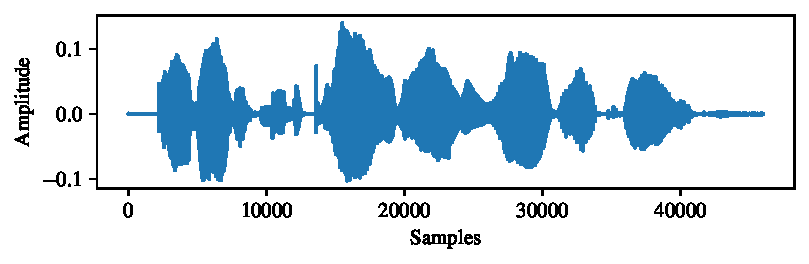
\includegraphics[width=.45\linewidth]{gfx/signal}
			    \label{fig:signal}
			    \caption{A raw waveform signal from the TIMIT dataset.}
			\end{figure}

		\paragraph{Pre-emphasis}

			In speech signals, high frequencies generally have smaller magnitudes than lower frequencies.
			To balance the magnitudes over the range of frequencies in the signal, we apply a pre-emphasis filter $y(t)$ on the waveform signal $x(t)$ defined in Equation \ref{eq:pre_emphasis}.
			\begin{equation}\label{eq:pre_emphasis}
				y(t) = x(t) - 0.97x(t-1)
			\end{equation}
			This procedure yields the additional benefit of improving the signal-to-noise ratio.
			An example of a pre-emphasized signal is given in Figure \ref{fig:signalemph}.
			\begin{figure}[ht]
				\centering
			    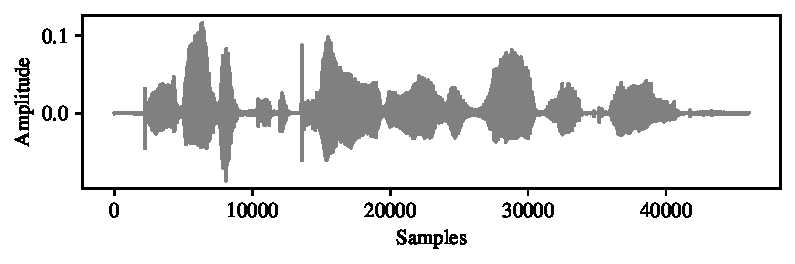
\includegraphics[width=.45\linewidth]{gfx/signalemph}
			    \label{fig:signalemph}
			    \caption[Pre-emphasis]{A signal after the pre-emphasis filter of Equation \ref{eq:pre_emphasis} was applied to it.}
			\end{figure}

		\paragraph{Framing}
			The waveforms, which are sampled at a rate $f_s$ of \SI{16}{\kHz}, cannot be directly used as input to the model, because they are too long---a typical sentence waveform contains in the order of tens of thousands of samples.
			Furthermore, the samples are not very informative, because they represent the sound wave of the uttered sound.
			These sounds are filtered by the shape of the vocal tract, which manifests itself in the envelope of the short time power spectrum of the sound.
			This power spectrum representation describes the power of the frequency components of the signal over a brief interval.
			We assume the frequency components to be stationary over short intervals---in contrast to the full sentence, which carries its meaning because it is non-stationary.
			Therefore, we transform the waveform signals into series of frequency coefficients of short-term power spectra.
			To obtain multiple short-term power spectra over the duration of the waveform, we slice it up into brief overlapping frames.


			Every 160 samples (equivalent to \SI{10}{ms}) of a pre-emphasized signal we take an interval frame of 400 samples (equivalent to \SI{25}{ms}).
			This means that the frames overlap by \SI{25}{ms}.
			The waveform is zero-padded such that the last frame also has 400 samples.
			By this process, we obtain signal frames $x_i(n)$, where $n$ ranges over 1--400, and $i$ ranges over the number of frames in the waveform.

			Then, we apply a Hamming window with the form
			\begin{equation}
				w\left[n\right] = a_0 - a_1\cos\left(\frac{2\pi n}{N-1}\right),
			\end{equation}
			where $N$ is the window length of 400 samples, $0 \leq n < N$, $a_0 = 0.53836$, and $a_1 = 0.46164$.
			A plot of this window is given in Figure \ref{fig:hamming}.
			\begin{figure}[ht]
				\centering
			    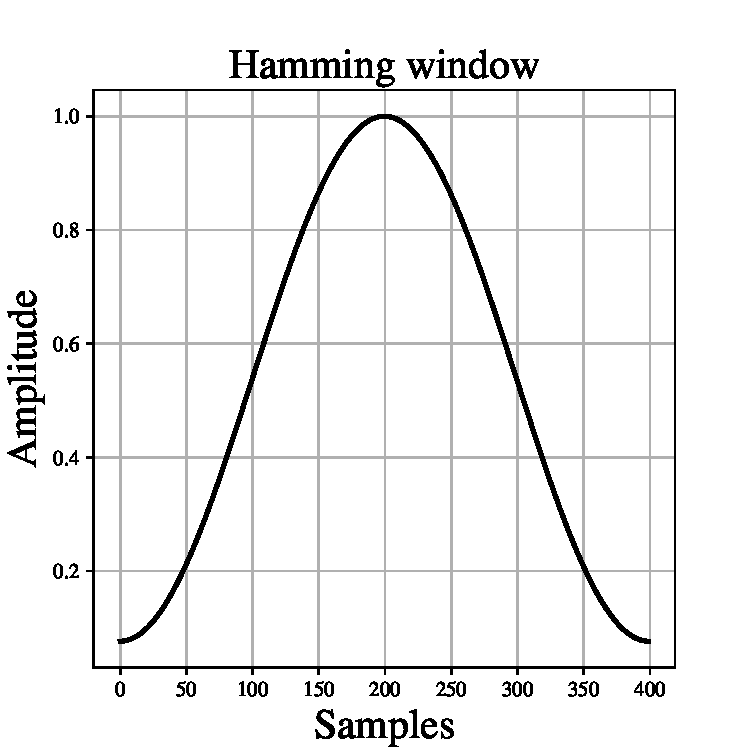
\includegraphics[width=.45\linewidth]{gfx/hamming}
			    \label{fig:hamming}
			    \caption{The magnitudes of the DFT of a frame.}
			\end{figure}
			This window is applied to reduce the spectral leakage, which manifests itself though sidelobes in the power spectra.
			Applying the Hamming window reduces the sidelobes to near-equiripple conditions \citep{SASPWEB2011}.\todo{plot for illustration}.

		\paragraph{Short-term power spectra}

			We obtain the power spectra $P_i$ for each frame by first taking the absolute $K$-point discrete Fourier transform (DFT) of the frame samples $x_i(n)$\todo{don't bother with eqn, just call mathbb(F)}
			\begin{equation}\label{eq:magframes}
				X_k = \left|\sum_{n=0}^{N-1}x_i(n)\cdot e^{-\frac{i2\pi}{N}kn}\right|,
			\end{equation}
			where $K=512$.
			This yields the magnitudes of the DCT of the frames (an example is illustrated in Figure \ref{fig:magframes}).
			\begin{figure}[ht]
				\centering
			    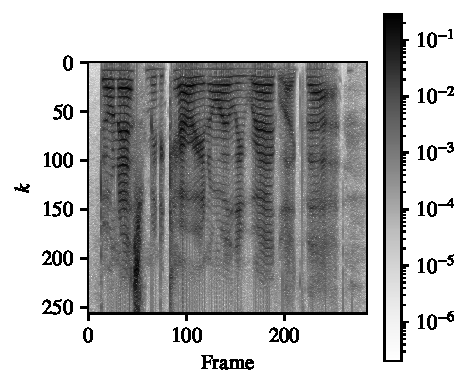
\includegraphics[width=.45\linewidth]{gfx/magframes}
			    \label{fig:magframes}
			    \caption{The magnitudes of the DFT of a frame.}
			\end{figure}

			We obtain the power spectrum using the equation

			\begin{equation}\label{eq:powframes}
				P = \frac{{X_k}^2}{K},
			\end{equation}
			an example of which is shown in Figure \ref{fig:powframes}.

			\begin{figure}[ht]
				\centering
			    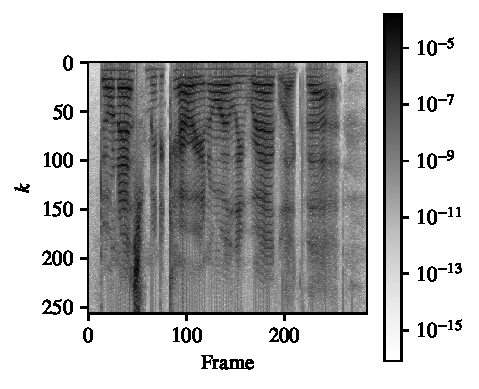
\includegraphics[width=.45\linewidth]{gfx/powframes}
			    \label{fig:powframes}
			    \caption{A power spectrum of a frame.}
			\end{figure}

		\paragraph{Mel filterbank}

			We then transform the short-term power spectra to Mel-spaced filterbanks.
			The Mel scale is a scale of pitches that are perceptually equal in distance \citep{stevens1937scale}.
			This is in contrast to the frequency measurement, in which the human cochlea can better distinguish lower frequencies better than higher ones.
			The aim of converting to the Mel scale is to make every filterbank coefficient feature equally informative, thereby improving the learning performance of the model.

			The Mel-spaced filterbank is a set of 40 triangular filters that we apply to each frame in $P$.

			To compute the Mel-spaced filterbank we choose lower and upper band edges of \SI{0}{\Hz} and $f_s/2 = \SI{8}{\kHz}$, respectively, and convert these to Mels using
			\begin{equation}
				m(f) = 2595\log_{10}\left(1 + \frac{f}{700}\right),
			\end{equation}
			where $f$ is the frequency in $\SI{}{\Hz}$.
			We obtain a lower band edge of 0 Mels and an upper band edge of approximately 2835 Mels.

			We begin obtaining the 40 filterbanks by spacing 42 points $\mathbf{m}$ linearly between these bounds (inclusive).
			Hence, we obtain 42 points spaced exclusively between the bounds.

			Then, we convert each point $m$ back to \SI{}{\Hz} using
			\begin{equation}
				f = 700\left(10^{m/2595}-1\right).
			\end{equation}
			We round each resulting Mel-spaced frequency $f$ to their nearest Fourier transform bin $b$ using
			\begin{equation}
				b = \lfloor(K+1)\mathbf{f}/fs\rfloor
			\end{equation}

			The resulting 40 filterbanks with their corresponding Mels and frequencies are listed in Table \ref{tab:mels}.

			The $i\textsuperscript{th}$ filter in filterbank $H_i$ is a triangular filter that has its lower boundary at $b_{i}$ \SI{}{\Hz}, its peak at $b_{i+1}$ \SI{}{\Hz}, and its upper boundary at $b_{i+2}$ \SI{}{\Hz}.\todo{not sure}
			For other frequencies, they are 0.
			Therefore, the filterbank can be described by
			\begin{equation}
				H_i(k) = \begin{cases}
					0 & k<b_i\\
					\frac{k-b_i}{b_{i+1}-b_i} & b_i\leq k < b_{i+1} \\
					1 & k = b_{i+1} \\
					\frac{b_{i+2} - k}{b_{i+2}-b_{i+1}} & b_{i+1} < k \leq b_{i+2}\\
					0 & b_{i+2} < k
				\end{cases},
			\end{equation}
			where $0 \leq k \leq \frac{K}{2}$.
			These Mel-spaced filters are shown in Figure \ref{fig:filterbank}.
			\begin{figure}[ht]
				\centering
			    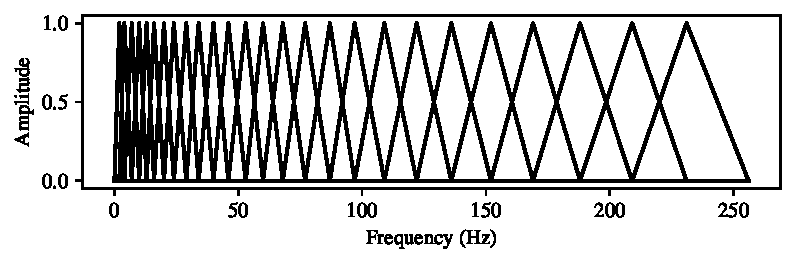
\includegraphics[width=.45\linewidth]{gfx/fbanks}
			    \label{fig:filterbank}
			    \caption{The Mel-spaced filterbanks.}
			\end{figure}

			We obtain a spectrogram $S$ of the frame (see \eg Figure \ref{fig:spectrogram}) after applying the filterbank to the short-term power spectrum.

			\begin{figure}[ht]
				\centering
			    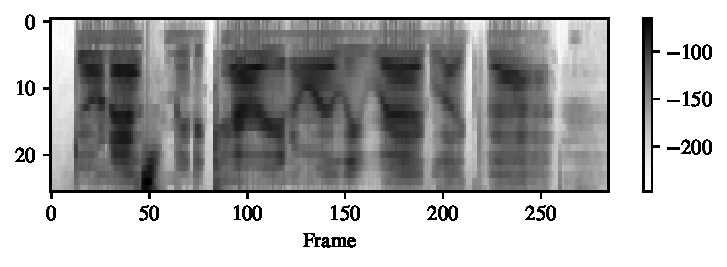
\includegraphics[width=.45\linewidth]{gfx/spectrogram}
			    \label{fig:spectrogram}
			    \caption{An example of a spectrogram.}
			\end{figure}

		\paragraph{Mel-frequency cepstral coefficients}

			We observe that the coefficients in the spectrograms are strongly correlated, which would negatively impact the learning performance of the model \todo{why?}.

			Therefore, we apply the DCT again to decorrelate the coefficients and obtain the power cepstrum $C$ of the speech frame:\todo{do we take absolute?}

			\begin{equation}\label{eq:magframes}
				C(n) = \left|\sum_{n=0}^{N-1}S(n)\cdot e^{-\frac{i2\pi}{N}kn}\right|.
			\end{equation}

			We discard the first coefficient in $C$, because it is the average power of the input signal and therefore carries little meaning.
			We also discard coefficients higher than 13, because they represent only fast changes in the spectrogram and increase the complexity of the input signal while adding increasingly less meaning to it. \todo{source?}
			An example of the remaining MFCC components is shown in Figure \ref{fig:mfccs}.

			\begin{figure}[ht]
				\centering
			    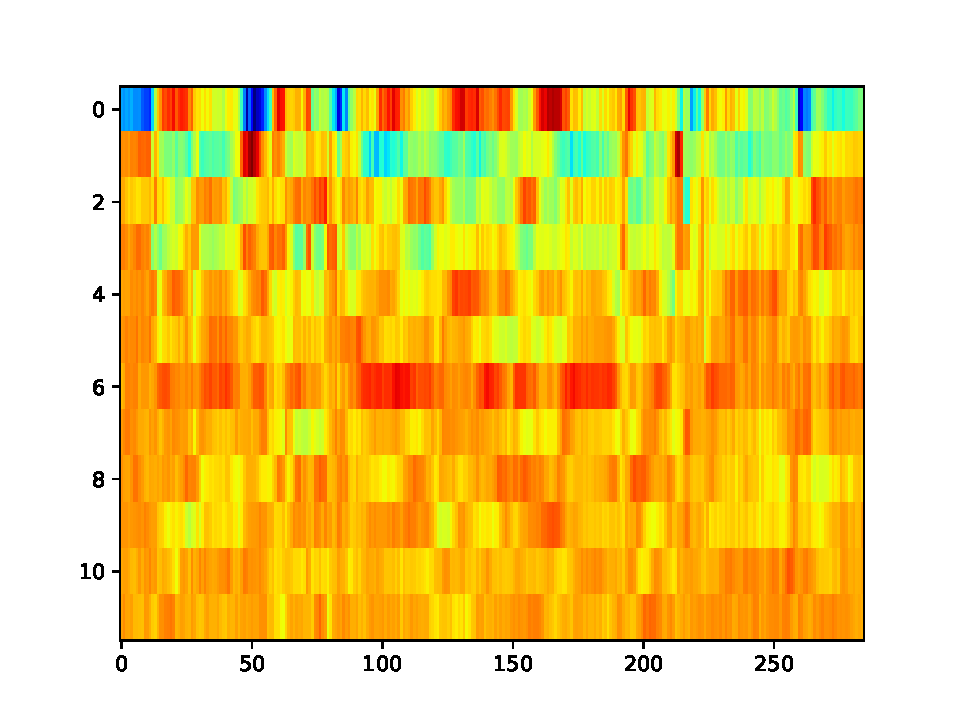
\includegraphics[width=.45\linewidth]{gfx/mfcc}
			    \label{fig:mfccs}
			    \caption{An example of Mel-frequency cepstral coefficients that are given as input to the system.}
			\end{figure}

			Finally, we balance the final MFCCs by centering them around 0 per frame.
			An example of the final MFCCs is given in \ref{fig:source_mfcc_target}.

		\paragraph{Target output}

			The target output of the model is a frame-wise representation of the phones that are uttered in a sentence.
			The TIMIT corpus contains text files indicating in what order phones occur in a sentence, and their starting and ending sample points.

			These phones are discretized into frames such that they align correctly with the MFCCs.
			They are represented in one-hot vector encoding.
			Since the dataset contains 61 different phones, this is also the length of these vectors.

			Figure \ref{fig:source_mfcc_target} illustrates the waveform data and its framewise aligned MFCCs and target output.

			\todo{side-by-side with original text and phonemes, label as fig:source\_mfcc\_target}



		\begin{figure}[ht]
		    \centering
		    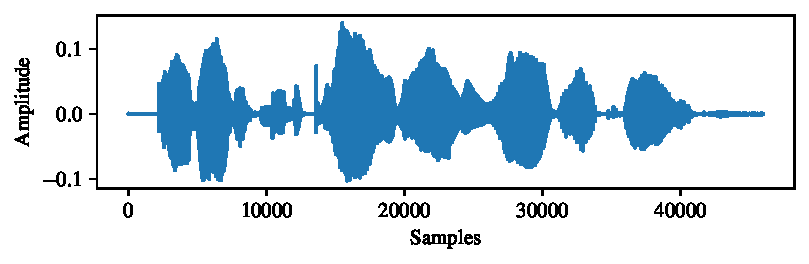
\includegraphics[width=.45\linewidth]{gfx/signal}\\
		    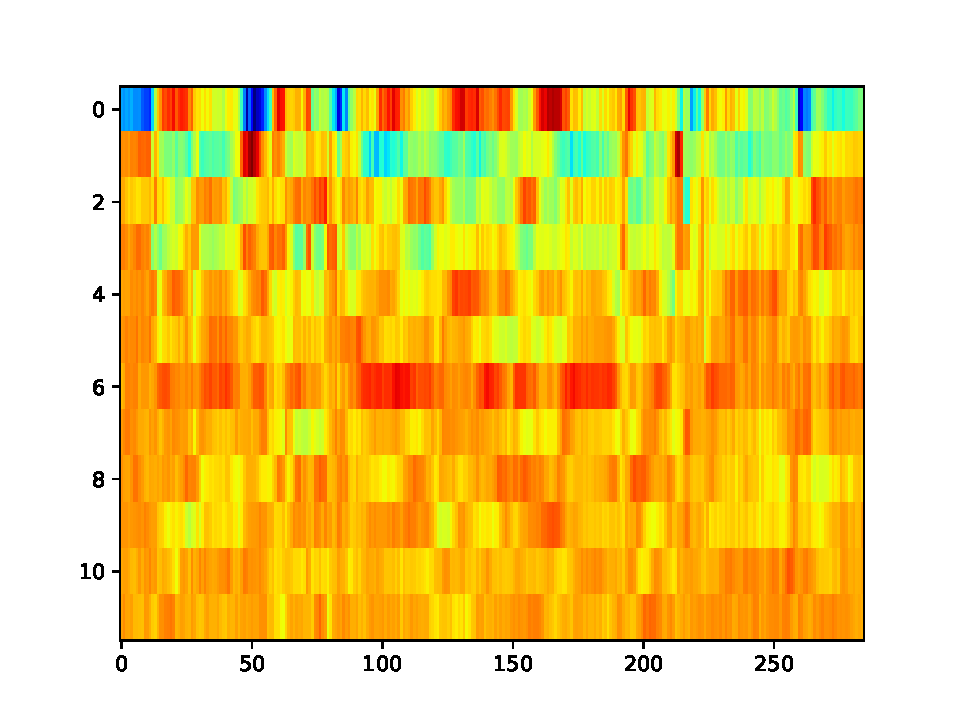
\includegraphics[width=.45\linewidth]{gfx/mfcc}\\
		    % 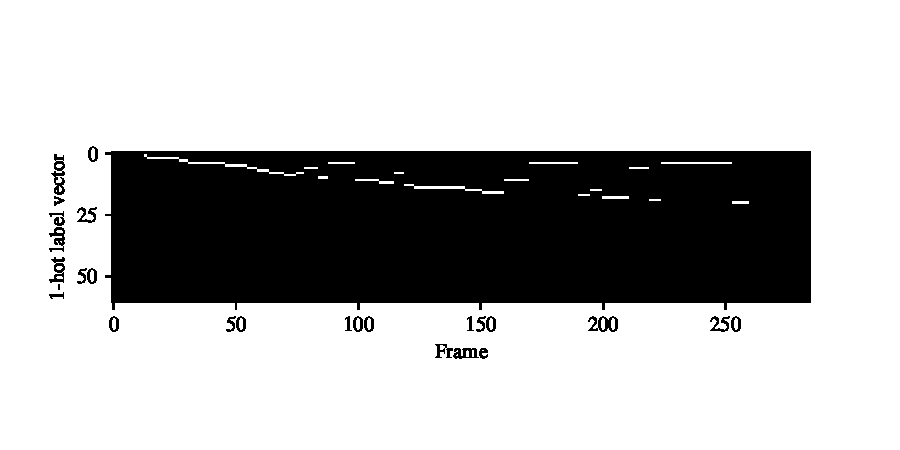
\includegraphics[width=.45\linewidth]{gfx/target}
		    \label{fig:source_mfcc_target}
		    \caption{An alignment of a sample signal with its MFCCs and target phones.}
		\end{figure}


%************************************************
\chapter{Method}\label{ch:method}
%************************************************
\section{Data Preprocessing}

	\subsection{The TIMIT speech corpus}
		TIMIT is a speech corpus that contains phonemically transcribed speech~\citep{garofolo1993darpa}, comprising 6300 sentences, 10 spoken by each of the 630 speakers.
		To include a broad range of dialects all speakers lived in 8 different geographical regions in the United States (as categorized in \citet{labov2008atlas}) during their childhood years.
		Table~\ref{tab:dialects} breaks down the precise composition of the dialect distribution.

		\begin{table}[ht]
		    \myfloatalign
		    \begin{tabularx}{\textwidth}{lrrr} \toprule
		        \tableheadline{Dialect region} & \tableheadline{\#Male}
		        & \tableheadline{\#Female} & \tableheadline{Total} \\ \midrule
		        % Phantoms take care of right-alignment (works iff monospaced digits)
		        1 (New England)   & 31 (63\%) & 18 (27\%) &  49  \phantom{0}(8\%)  \\
		        2 (Northern)      & 71 (70\%) & 31 (30\%) & 102 (16\%) \\
		        3 (North Midland) & 79 (67\%) & 23 (23\%) & 102 (16\%) \\
		        4 (South Midland) & 69 (69\%) & 31 (31\%) & 100 (16\%) \\
		        5 (Southern)      & 62 (63\%) & 36 (37\%) &  98 (16\%) \\
		        6 (New York City) & 30 (65\%) & 16 (35\%) &  46  \phantom{0}(7\%)  \\
		        7 (Western)       & 74 (74\%) & 26 (26\%) & 100 (16\%) \\
		        8                 & 22 (67\%) & 11 (33\%) &  33  \phantom{0}(5\%)  \\
		        \midrule
		        All  & 438 (70\%) & 192 (30\%) & 630 (100\%) \\
		        \bottomrule
		    \end{tabularx}
		    \caption[TIMIT Dialect Regions]{Distribution of speakers' dialect regions and sexes. Speakers of the innominate dialect region 8 relocated often during their childhood.}  \label{tab:dialects}
		\end{table}

		The sentence text can be categorized into 2 \emph{dialect} sentences, 450 \emph{phonetically compact} sentences, and 1890 \emph{phonetically diverse} sentences.

		The dialect sentences, which are spoken by all speakers, are designed to expose the dialectical variants of the speakers.
		The phonetically compact sentences are designed to include many pairs of phones.
		The phonetically diverse sentences are taken from the Brown Corpus~\citep{kucera1967computational} and the Playwrights Dialog~\citep{hultzsch1964tables} in order to maximize the number of allophones (\ie, different phones used to pronounce the same phoneme).
		Table~\ref{tab:types} lists an overview of the distribution of the number of speakers per sentence type.

		\begin{table}[ht]
		    \myfloatalign
		    \begin{tabularx}{\textwidth}{lrrrr} \toprule
		        \tableheadline{Sentence type} & \tableheadline{\#Sentences}
		        & \tableheadline{\#Speakers} & \tableheadline{Total} \\ \midrule
		        % Phantoms take care of right-alignment (works iff monospaced digits)
		        Dialect & 2    & 630 & 1260\\
		        Compact & 450  & 7   & 3150 \\
		        Diverse & 1890 & 1   & 1890 \\
		        \midrule
		        Total   & 2342 &     & 6300 \\
		        \bottomrule
		    \end{tabularx}
		    \caption[TIMIT Sentence Types]{Distribution of sentence types.}
		    \label{tab:types}
		\end{table}

		Each of the sentences is encoded in as a waveform signal in \texttt{.wav} format, and is accompanied by a corresponding text file indicating which phones are pronounced in the waveform, and between which pairs of sample points.

	\subsection{Data splitting}
		The TIMIT dataset is split into a training, validation and testing set as in \citet{graves2005framewise} and \citet{bellec2020solution}.
		The training set is used to train the network synaptic weights according to the e-prop algorithm.
		The validation set is used to obtain a well-performing set of hyperparameters.
		The testing set is used to evaluate the performance of the network after the hyperparameters are obtained.

		The TIMIT corpus documentation offers a suggested partitioning of the training and testing data, which is based on the following criteria:
		\begin{enumerate}
			\item 70\%--80\% of the data is used for training, and the remaining 20\%--30\% for testing.
			\item No speaker appears in both the training and testing portions.
			\item Both subsets include at least 1 male and 1 female speaker from every dialect region.
			\item There is a minimal overlap of text material in the two subsets.
			\item The test set should contain all phonemes in as many allophonic contexts as possible.
		\end{enumerate}
		In accordance with these criteria, the TIMIT corpus includes a ``core'' test set that contains 2 male speakers and 1 female speaker from each dialect, summing up to 24 speakers.
		Each of these speakers read a different set of 5 phonetically compact sentences, and 3 phonetically diverse sentences that were unique for each speaker.
		Consequently, the test set comprises 192 sentences ($24\times(5+3)$) and was selected such that it contains at least one occurrence of each phoneme.
		In this report, the TIMIT core test set is used, thereby meeting the criteria listed above.

		The remaining 4096 sentences are randomly partitioned into 3696 training sentences and 400 validation sentences.

	\subsection{Engineering features}

		The data preprocessing pipeline is similar to that used in \citet{fayek2016}, which can be summarized by applying a pre-emphasis filter on the waveforms, then slicing the waveform in short frames, taking their short-term power spectra, computing 26 filterbanks, and finally obtain 12 Mel-Frequency Cepstrum Coefficients (MFCCs).
		Then, these MFCCs are aligned with the phones found in the TIMIT dataset.
		An example of a waveform signal is given in Figure \ref{fig:signal}.
			\begin{figure}[ht]
				\centering
			    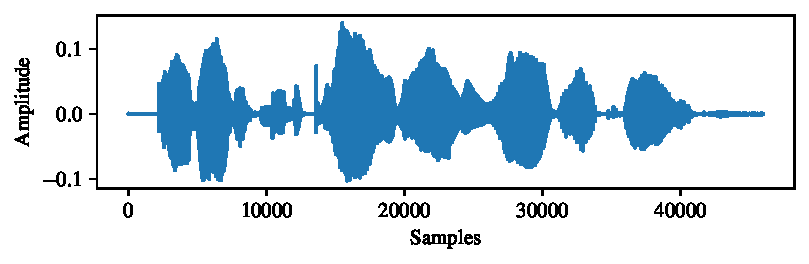
\includegraphics[width=\linewidth]{gfx/signal}
			    \caption{A raw waveform signal from the TIMIT dataset.}
			    \label{fig:signal}
			\end{figure}

		\paragraph{Pre-emphasis}

			In speech signals, high frequencies generally have smaller magnitudes than lower frequencies.
			To balance the magnitudes over the range of frequencies in the signal, a pre-emphasis filter $y(t)$ is applied on the waveform signal $x(t)$ defined in Equation \ref{eq:pre_emphasis}.
			\begin{equation}\label{eq:pre_emphasis}
				y(t) = x(t) - 0.97x(t-1)
			\end{equation}
			This procedure yields the additional benefit of improving the signal-to-noise ratio.
			An example of a pre-emphasized signal is given in Figure \ref{fig:signalemph}.
			\begin{figure}[ht]
				\centering
			    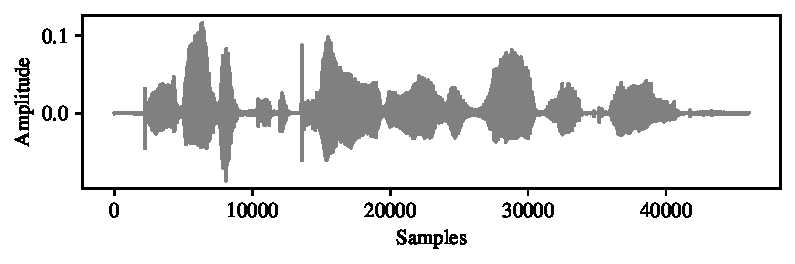
\includegraphics[width=\linewidth]{gfx/signalemph}
			    \caption[Pre-emphasis]{A signal after the pre-emphasis filter of Equation \ref{eq:pre_emphasis} was applied to it.}
			    \label{fig:signalemph}
			\end{figure}

		\paragraph{Framing}
			The waveforms, which are sampled at a rate $f_s$ of \SI{16}{\kHz}, cannot be directly used as input to the model, because they are too long---a typical sentence waveform contains in the order of tens of thousands of samples.
			Furthermore, the samples are not very informative, because they represent the sound wave of the uttered sound.
			These sounds are filtered by the shape of the vocal tract, which manifests itself in the envelope of the short time power spectrum of the sound.
			This power spectrum representation describes the power of the frequency components of the signal over a brief interval.
			The frequency components are assumed to be stationary over short intervals---in contrast to the full sentence, which carries its meaning because it is non-stationary.
			Therefore, the waveform signals are transformed into series of frequency coefficients of short-term power spectra.
			To obtain these multiple short-term power spectra over the duration of the waveform, it is sliced into brief overlapping frames.

			Every 160 samples (equivalent to \SI{10}{ms}) of a pre-emphasized signal, an interval frame of 400 samples (equivalent to \SI{25}{ms}) is extracted.
			This means that the frames overlap by \SI{25}{ms}.
			The waveform is zero-padded such that the last frame also has 400 samples.
			By this process, signal frames $x_i(n)$ are obtained, where $n$ ranges over 1--400, and $i$ ranges over the number of frames in the waveform.

			Then, a Hamming window with the form
			\begin{equation}\label{eq:hamming}
				w\left[n\right] = a_0 - a_1\cos\left(\frac{2\pi n}{N-1}\right),
			\end{equation}
			is applied where $N$ is the window length of 400 samples, $0 \leq n < N$, $a_0 = 0.53836$, and $a_1 = 0.46164$.
			A plot of this window is given in Figure \ref{fig:hamming}.
			\begin{figure}[ht]
				\centering
			    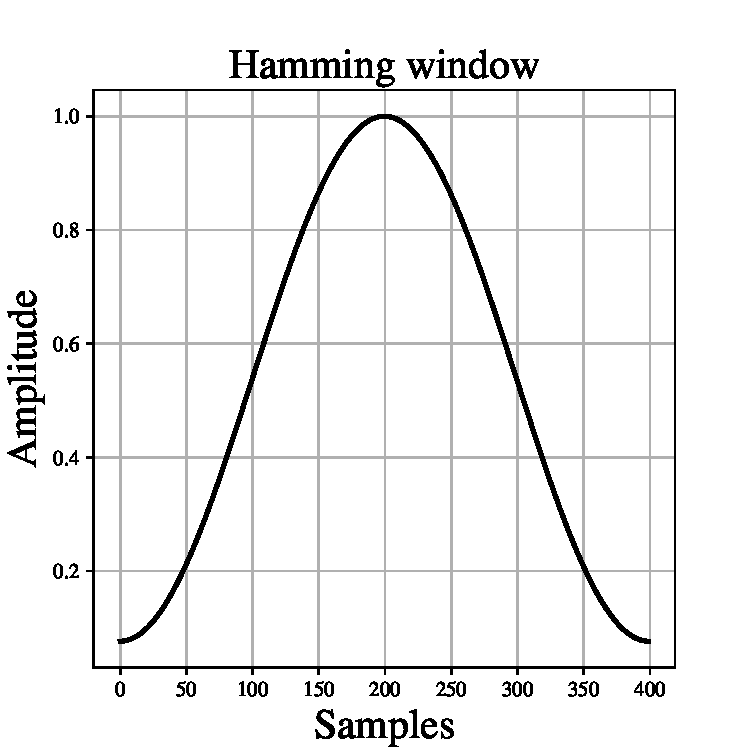
\includegraphics[width=0.45\linewidth]{gfx/hamming}
			    \caption{The form of the Hamming window applied on signal frames to reduce spectral leakage.}
			    \label{fig:hamming}
			\end{figure}
			This window is applied to reduce the spectral leakage, which manifests itself though sidelobes in the power spectra.
			Applying the Hamming window reduces the sidelobes to near-equiripple conditions, minimizing the leakage \citep{SASPWEB2011}.

		\paragraph{Short-term power spectra}

			The power spectra $P_i$ are obtained for each frame by first taking the absolute $K$-point discrete Fourier transform (DFT) of the frame samples $x_i(n)$:
			% \todo{don't bother with eqn, just call mathbb(F)}
			\begin{equation}
				X_k = \left|\sum_{n=0}^{N-1}x_i(n)\cdot e^{-\frac{i2\pi}{N}kn}\right|,
			\end{equation}
			where $K=512$.
			This yields the magnitudes of the DCT of the frames (an example is illustrated in Figure \ref{fig:magframes}).
			\begin{figure}[ht]
				\centering
			    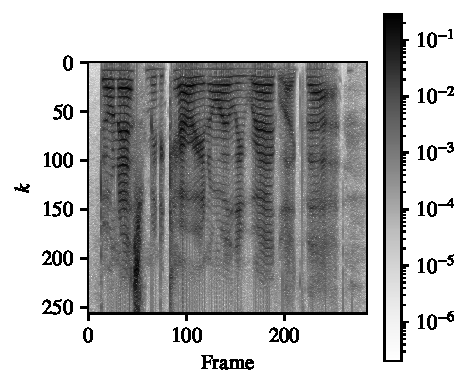
\includegraphics[width=0.45\linewidth]{gfx/magframes}
			    \caption{The magnitudes of the DFT of a frame.}
			    \label{fig:magframes}
			\end{figure}

			The power spectra are obtained using the equation
			\begin{equation}\label{eq:powframes}
				P = \frac{{X_k}^2}{K},
			\end{equation}
			an example of which is shown in Figure \ref{fig:powframes}.

			\begin{figure}[ht]
				\centering
			    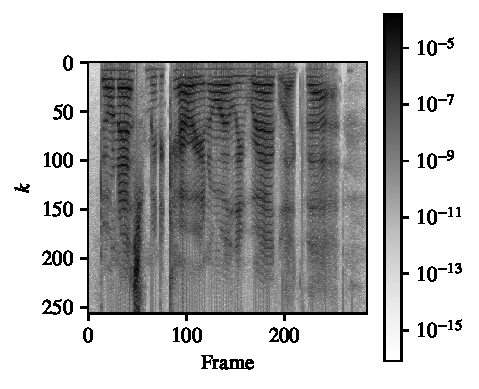
\includegraphics[width=0.45\linewidth]{gfx/powframes}
			    \caption{The power spectrum of a frame.}
			    \label{fig:powframes}
			\end{figure}

		\paragraph{Mel filterbank}

			The short-term power spectra are then transformed to Mel-spaced filterbanks.
			The Mel scale is a scale of pitches that are perceptually equal in distance \citep{stevens1937scale}.
			This is in contrast to the frequency measurement, in which the human cochlea can better distinguish lower frequencies better than higher ones.
			The aim of converting to the Mel scale is to make every filterbank coefficient feature equally informative, thereby improving the learning performance of the model.

			The Mel-spaced filterbank is a set of 40 triangular filters that we apply to each frame in $P$.

			To compute the Mel-spaced filterbank, lower and upper band edges of respectively \SI{0}{\Hz} and $f_s/2 = \SI{8}{\kHz}$ are selected, and convert these to Mels using
			\begin{equation}
				m(f) = 2595\log_{10}\left(1 + \frac{f}{700}\right),
			\end{equation}
			where $f$ is the frequency in $\SI{}{\Hz}$.
			This yields a lower band edge of 0 Mels and an upper band edge of approximately 2835 Mels.

			The 40 filterbanks are obtained by first spacing 42 points $\mathbf{m}$ linearly between these bounds (inclusive), thereby obtaining 40 points spaced exclusively between the bounds.

			Then, each point $m$ is converted back to \SI{}{\Hz} using
			\begin{equation}
				f = 700\left(10^{m/2595}-1\right).
			\end{equation}
			Resulting Mel-spaced frequencies $f$ are rounded to their nearest Fourier transform bin $b$ using
			\begin{equation}
				b = \lfloor(K+1)\mathbf{f}/fs\rfloor.
			\end{equation}

			The resulting 40 filterbanks with their corresponding Mels and frequencies are listed in Table \ref{tab:mels}.

			The $i\textsuperscript{th}$ filter in filterbank $H_i$ is a triangular filter that has its lower boundary at $b_{i}$ \SI{}{\Hz}, its peak at $b_{i+1}$ \SI{}{\Hz}, and its upper boundary at $b_{i+2}$ \SI{}{\Hz}.
			For other frequencies, they are 0.
			Therefore, the filterbank can be described by
			\begin{equation}
				H_i(k) = \begin{cases}
					0 & k<b_i\\
					\frac{k-b_i}{b_{i+1}-b_i} & b_i\leq k < b_{i+1} \\
					1 & k = b_{i+1} \\
					\frac{b_{i+2} - k}{b_{i+2}-b_{i+1}} & b_{i+1} < k \leq b_{i+2}\\
					0 & b_{i+2} < k
				\end{cases},
			\end{equation}
			where $0 \leq k \leq \frac{K}{2}$.
			These Mel-spaced filters are shown in Figure \ref{fig:filterbank}.
			\begin{figure}[ht]
				\centering
			    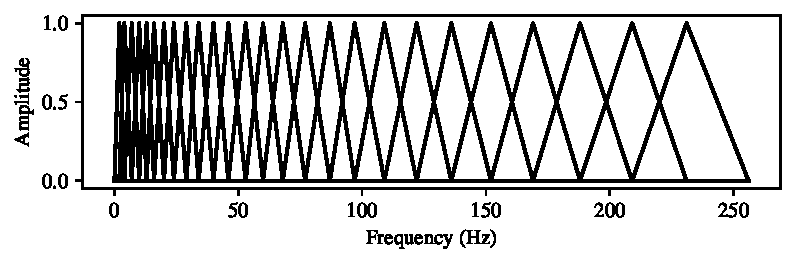
\includegraphics[width=\linewidth]{gfx/fbanks}
			    \caption{The Mel-spaced filterbanks.}
			    \label{fig:filterbank}
			\end{figure}

			After applying the filterbank to the short-term power spectrum, a spectrogram $S$ of the frame (see \eg~Figure \ref{fig:spectrogram}) is obtained.

			\begin{figure}[ht]
				\centering
			    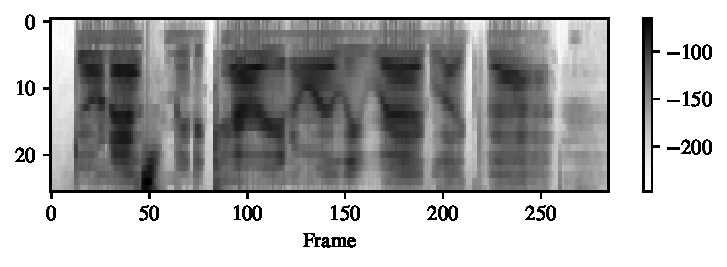
\includegraphics[width=\linewidth]{gfx/spectrogram}
			    \caption{An example of a frame spectrogram.}
			    \label{fig:spectrogram}
			\end{figure}

		\paragraph{Mel-frequency cepstral coefficients}

			Coefficients in the spectrograms are strongly correlated, which would negatively impact the learning performance of the model.
			Therefore, the DCT is applied again to decorrelate the coefficients and obtain the power cepstrum $C$ of the speech frame:

			\begin{equation}
				C(n) = \left|\sum_{n=0}^{N-1}S(n)\cdot e^{-\frac{i2\pi}{N}kn}\right|.
			\end{equation}

			The first coefficient in $C$ is discarded, because it indicates the average power of the input signal and therefore carries little meaning.
			Coefficients higher than 13 are also discarded, because they represent only fast changes in the spectrogram and increase the complexity of the input signal while adding increasingly less meaning to it.

			Then, the final MFCCs are balanced by centering each frame around the value 0.
			An example of the final MFCCs is given in Figure \ref{fig:source_mfcc_target}.

		\paragraph{Target output}

			The target output of the model is a frame-wise representation of the phones that are uttered in a sentence.
			The TIMIT corpus contains text files indicating in what order phones occur in a sentence, and their starting and ending sample points.

			These phones are discretized into frames such that they align correctly with the MFCCs.
			They are represented in one-hot vector encoding.
			Since the dataset contains 61 different phones, this is also the length of these vectors.

			Figure \ref{fig:source_mfcc_target} illustrates the waveform data and its frame-wise aligned MFCCs and target output.
			Note that the full dataset of features is standardized per channel; feature channels are first centered around 0, and then divided by their standard deviations.

			\begin{figure}[bth]
			    \myfloatalign
			    \subfloat[Input signal.]
			    {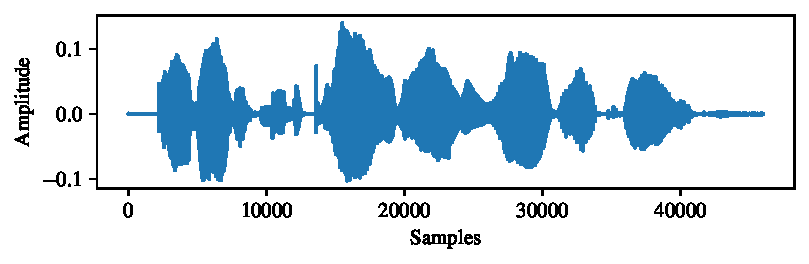
\includegraphics[width=\linewidth]{gfx/signal}} \\
			    \subfloat[MFCCs centered around 0 per channel.]
			    {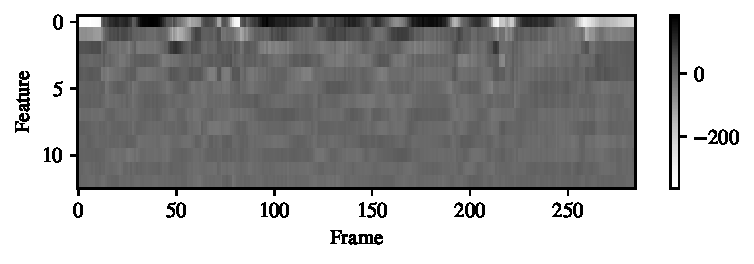
\includegraphics[width=\linewidth]{gfx/norm_mfcc}} \\
			    \subfloat[Target signal encoded as a one-hot vector changing over time.]
			    {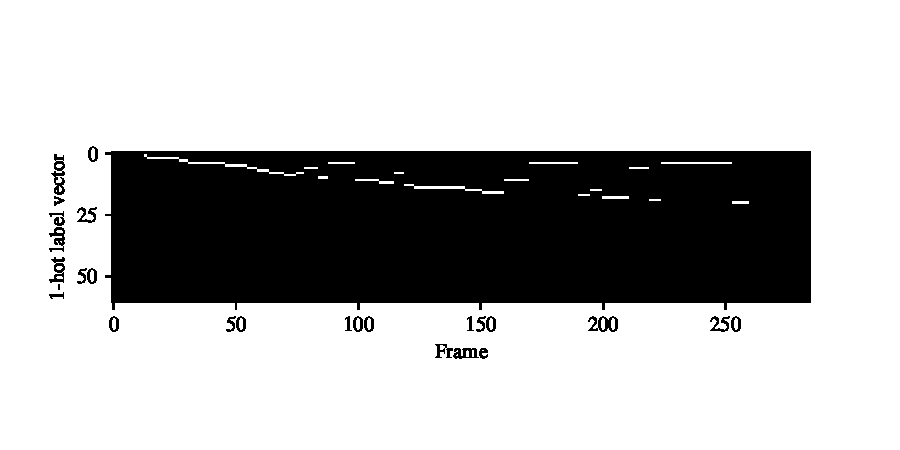
\includegraphics[width=\linewidth]{gfx/target}}
			    \caption[Input/features/targets]{An alignment of a sample signal with its MFCCs features and target phones.}\label{fig:source_mfcc_target}
			\end{figure}


\section{Enhancing e-prop}

	This report examines two types of enhancements to applying the e-prop learning algorithm on the TIMIT dataset.

	The first type is the effect of the neuron model; particularly, the effect of including STDP behavior is analyzed.
	The second type is the effect of a multi-layered architecture.

	\subsection{Multi-layer architecture}

		% \begin{figure}[bth]
		%     \myfloatalign
		%     \subfloat[A single-layer network. At time step $t$, the feature vector $x^t$ is fed to a mixed network of LIF and ALIF neurons. Then, the output weights $W^\text{out}$ transform the neuron's observable values into an output value $y^t$, such that the softmax function can be applied to obtain the logits $\pi^t$. The trainable e-prop connections (colored red) are updated by applying the broadcast weights $B$ on the learning signal $L^t$.]
		%     {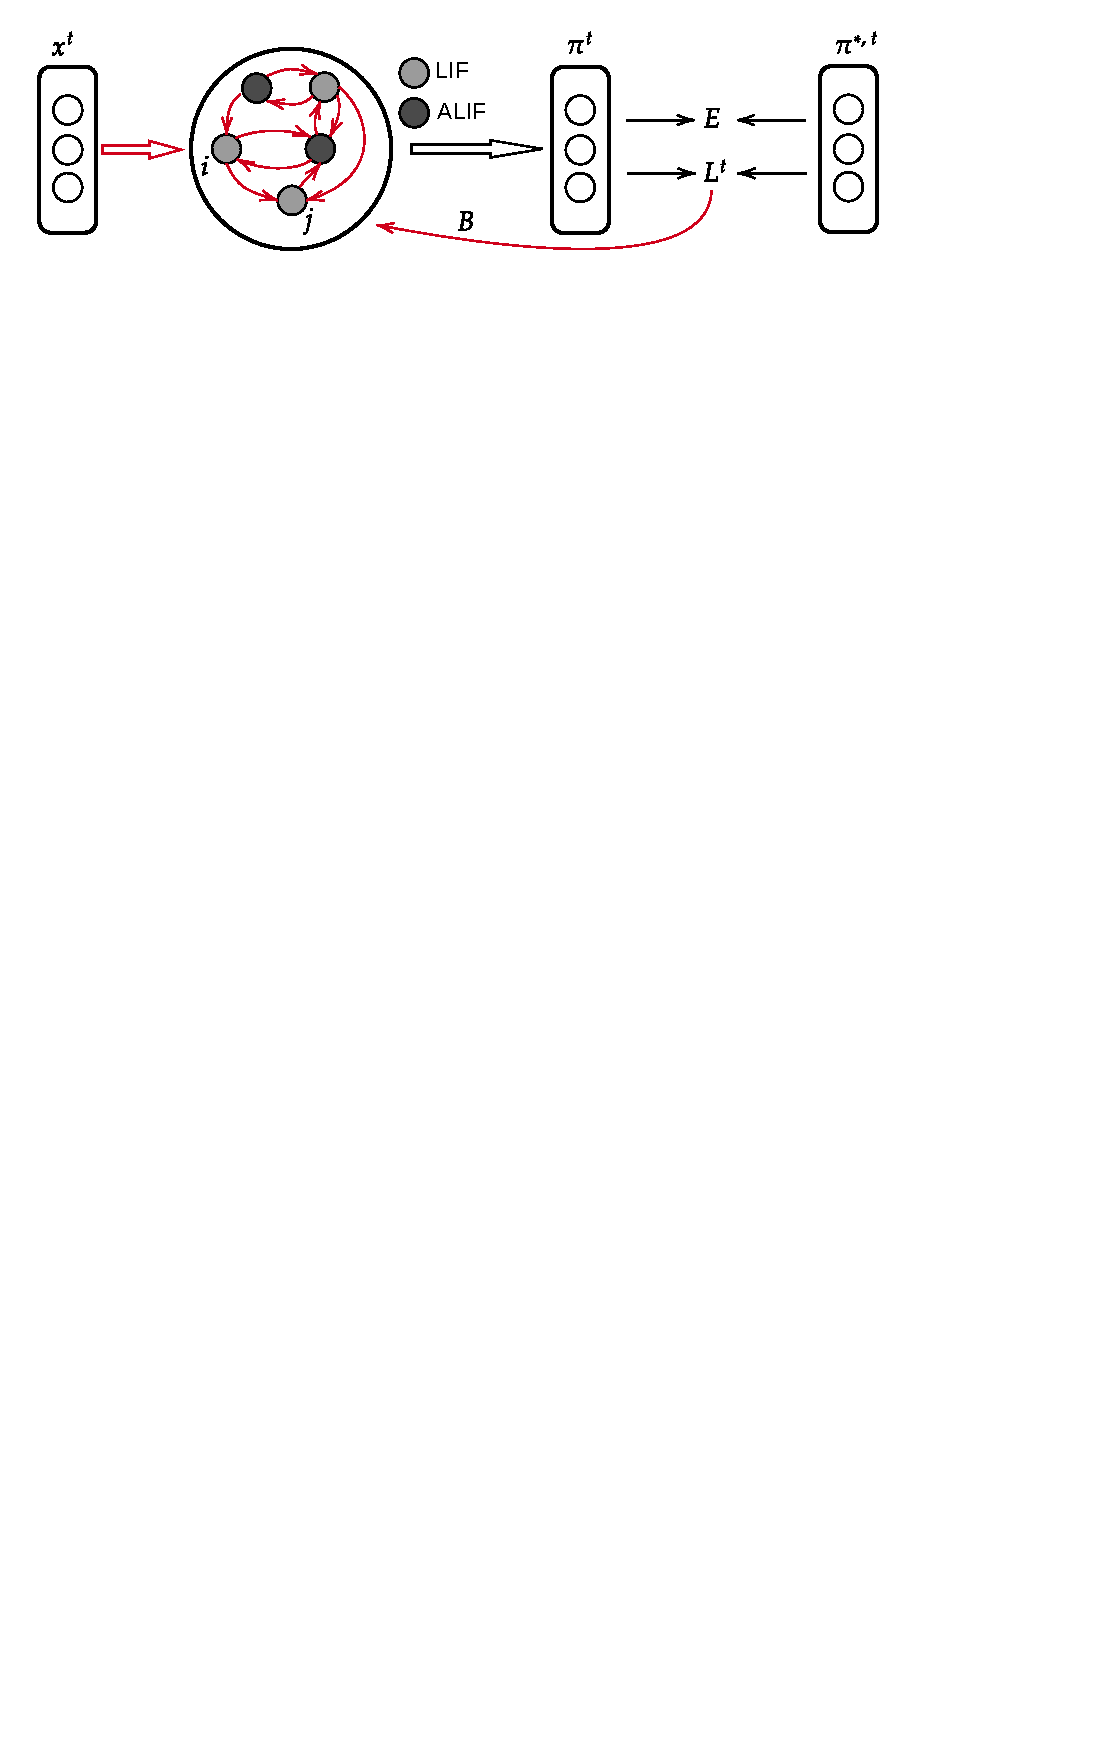
\includegraphics[trim=0 25cm 0 0, clip, width=\linewidth]{gfx/Singlelayer}} \\
		%     \subfloat[A multi-layer network with two stacked recurrent layers. ]
		%     {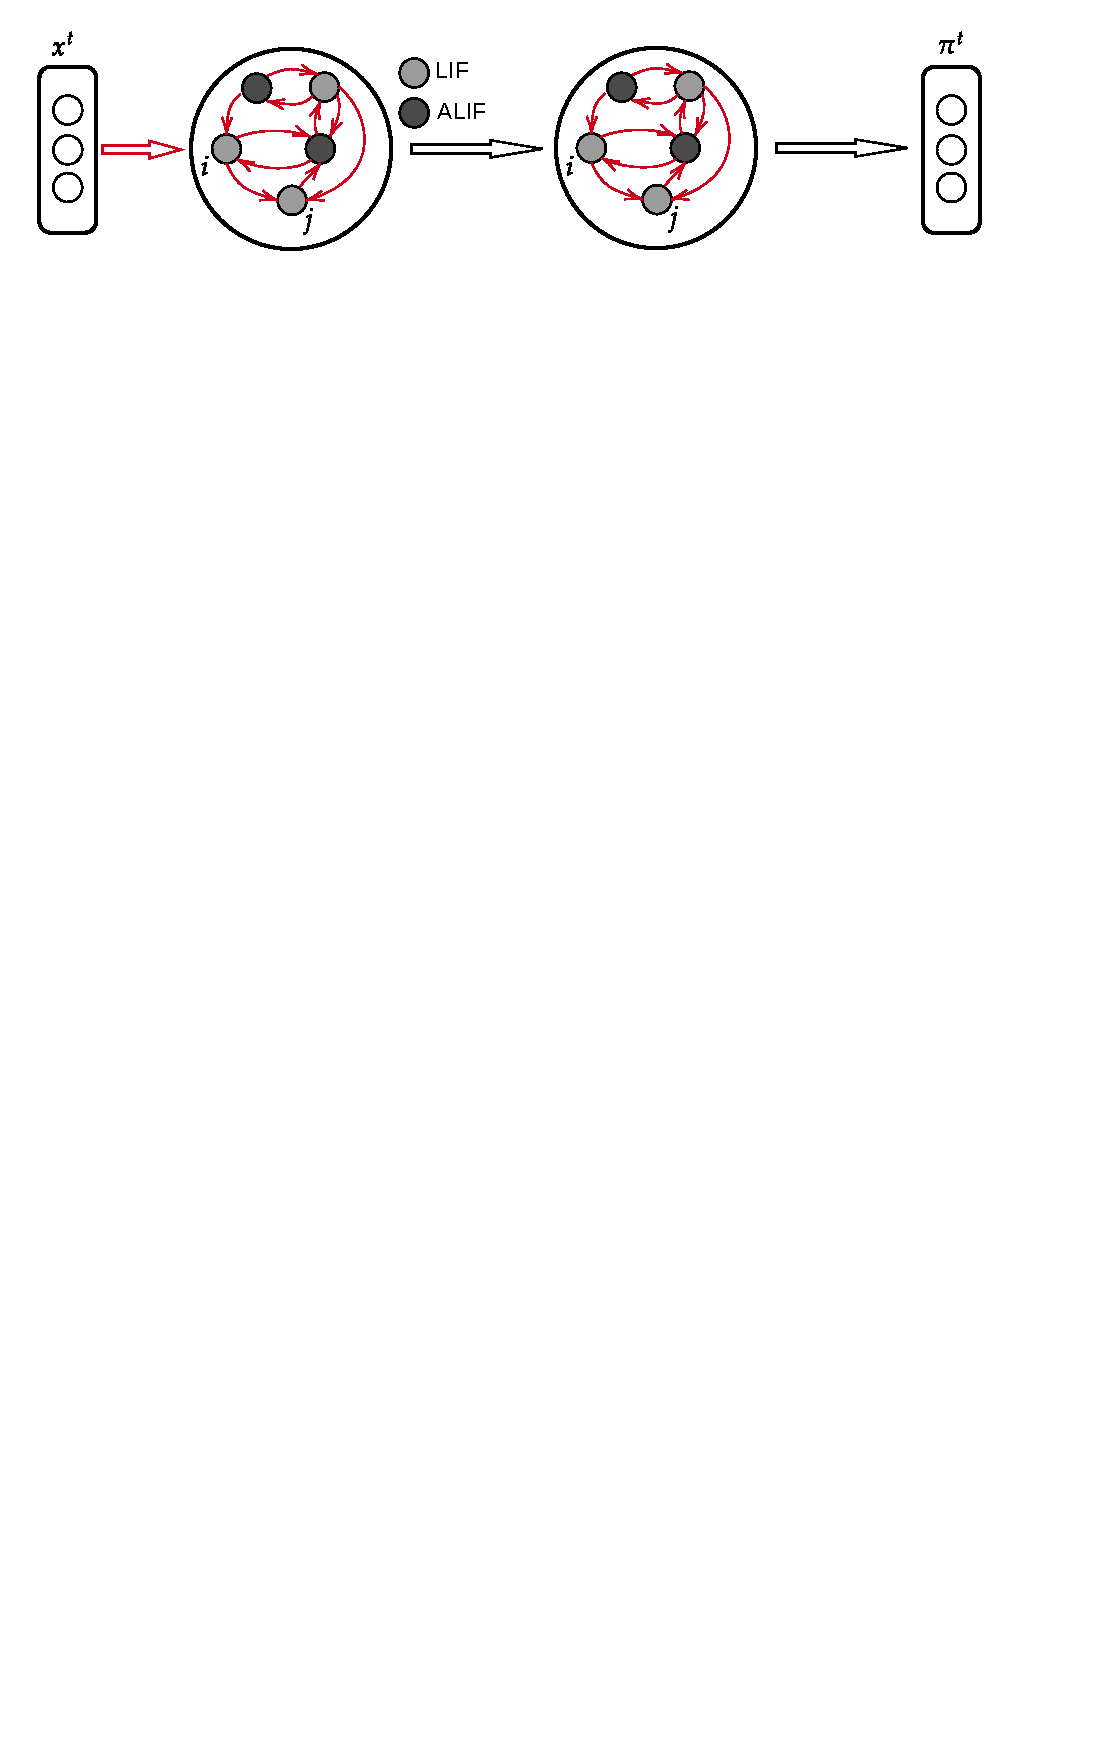
\includegraphics[trim=0 25cm 0 0, clip, width=\linewidth]{gfx/Multilayer}}
		%     \caption[Input/features/targets]{An illustration of a single-layer and multi-layer network architecture.}\label{fig:topology}
		% \end{figure}
		\begin{figure}[!ht]
		    \myfloatalign
		    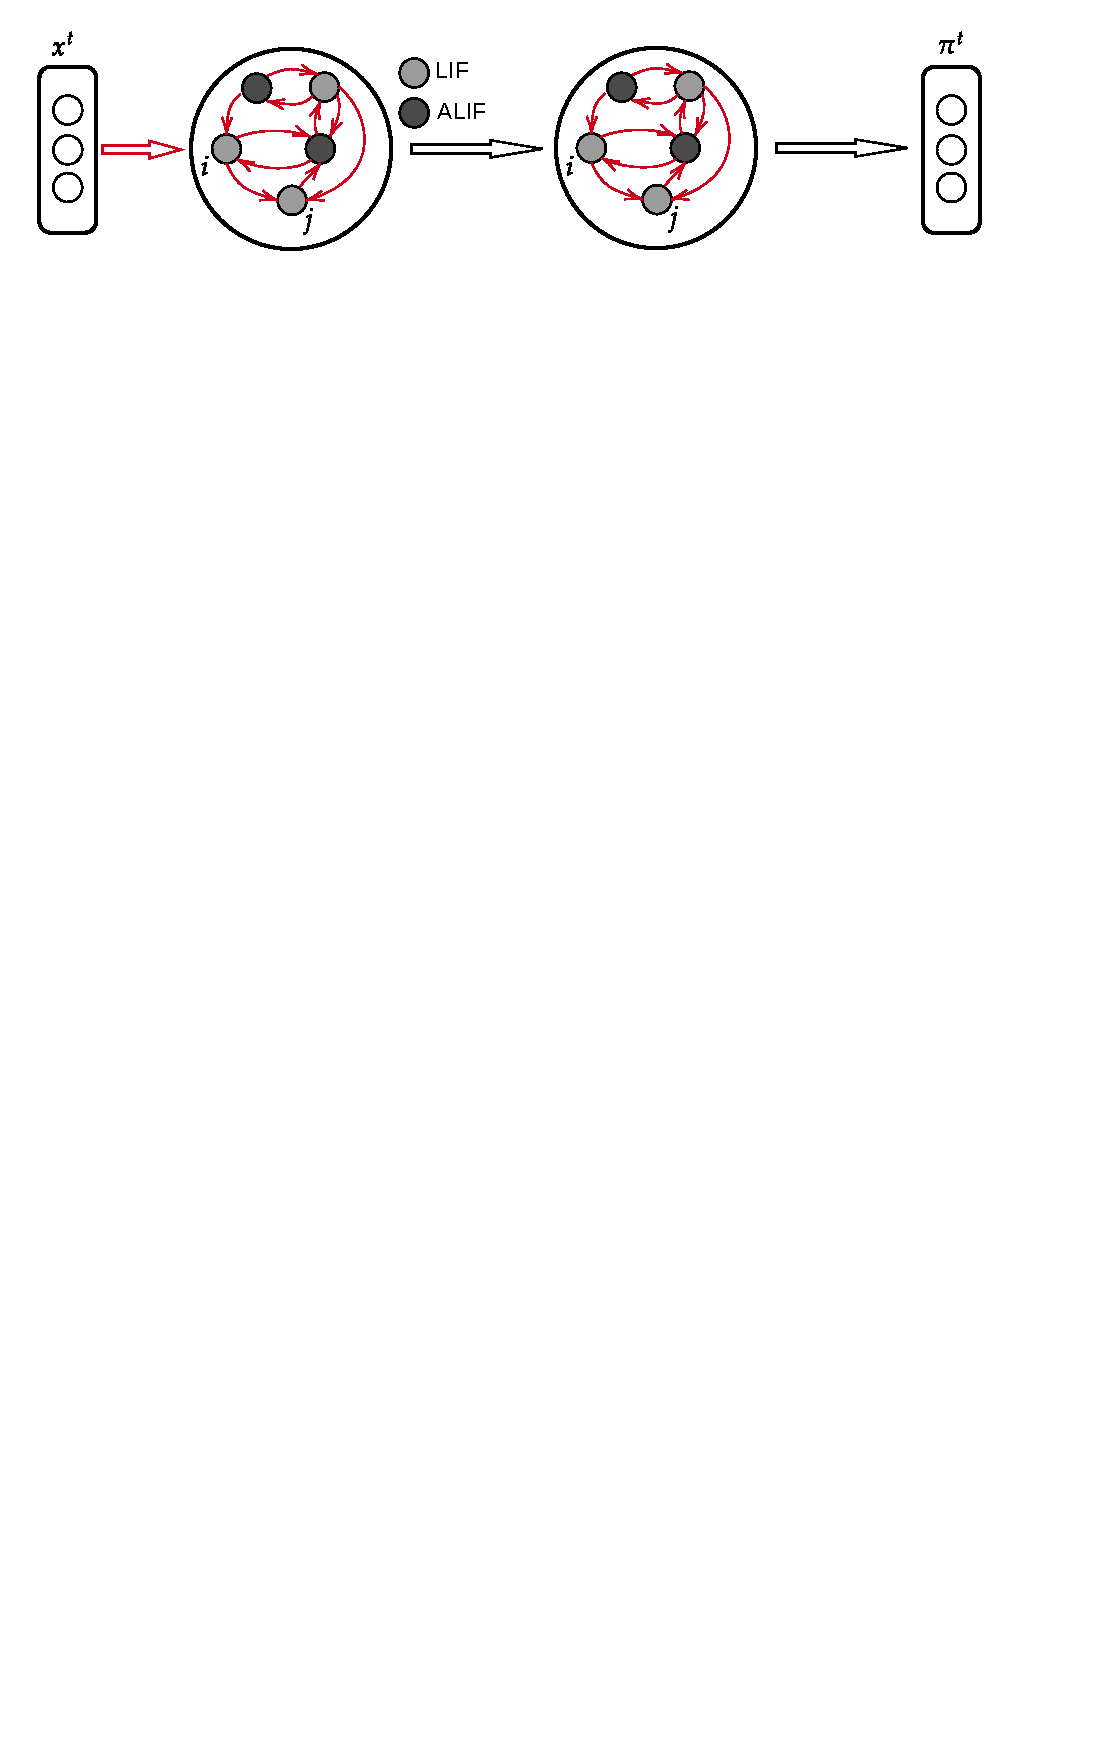
\includegraphics[trim=0 25cm 0 0, clip, width=\linewidth]{gfx/Multilayer}
		    \caption[Multi-layer illustration.]{An illustration of a multi-layer network architecture. Some details shown in Figure (\ref{fig:topology-sl} b) are omitted for clarity}
		    \label{fig:topology-ml}
		  \end{figure}

		The multi-layer e-prop architecture can be described in the same formal model as its single-layer counterpart, in which the hidden state is based on temporally (i.e., online) and spatially locally available information at a neuron $j$:

        \begin{equation}
        \mathbf{h}^t_j = M\left(\mathbf{h}_j^{t-1}, \mathbf{z}^{t-1}, \mathbf{x}^t, \mathbf{W}_j\right).\tag{\ref{eq:model} revisited}
        \end{equation}
        For the multi-layer architecture, however, neurons in deeper layers no longer depend on the input, but on the observable states of the previous layer at the same time step, such that at every time step, a full pass through the network is made.
        We modify the indexing notation accordingly, in order to directly refer to neurons and weights in a particular layer $r \in [1\mathrel{{.}\,{.}}\nobreak R]$:
        \begin{equation}\label{eq:ml_model}
        \mathbf{h}^t_{rj} = \begin{cases}
        M\left(\mathbf{h}_{rj}^{t-1}, \mathbf{z}_r^{t-1}, \mathbf{x}^t, \mathbf{W}_{rj}\right)       & \mbox{if } r = 1\\
        M\left(\mathbf{h}_{rj}^{t-1}, \mathbf{z}_r^{t-1}, \mathbf{z}_{r-1}^t, \mathbf{W}_{rj}\right) & \mbox{otherwise,}
        \end{cases}
        \end{equation}
        where $\mathbf{h}^t_{rj}$ (resp. $z^t_{rj}$) is the hidden state (resp. observable state) of a neuron $j$ in layer $r$. and $\mathbf{W}_{rj} = \mathbf{W}^\text{in}_{rj} \cup \mathbf{W}^\text{rec}_{rj}$ is the set of afferent weights to neuron $j$ in layer $r$.

        Similarly, the observable state can be modeled by
        \begin{equation}\label{eq:ml_model_obs}
        z^t_{rj} = f\left(\mathbf{h}_{rj}^t\right)
        \end{equation}
        and the network output by
        \begin{equation}
        y^t_k = \kappa y^{t-1}_k + \sum_{j,r}W^\text{out}_{rkj}z_{rj}^t + b_k,
        \end{equation}
        where $W^\text{out}_{rkj}$ is a weight between neuron $j$ in layer $r$ and output neuron $k$.
        Note that the summation over $r$ entails that the output layer is connected to all neurons in all layers in the network.
        This allows trainable broadcast weights in earlier layers, such as those found in symmetric and adaptive e-prop.

        \paragraph{Multi-layer ALIF neurons}
        An ALIF neuron in a multi-layer architecture is similar to one in a single-layer architecture (see Section \ref{sec:alif}).
        The only difference, apart from the layer indexing, is its activity update.
        For a multi-layer ALIF neuron, the activity value is given by
        \begin{equation}\label{eq:ml_alifV}
        v^{t+1}_{rj} = \alpha v_{rj}^t + \sum_{i\neq j}W^\text{rec}_{rji}z_i^t + \sum_i W^\text{in}_{rji}I - z_{rj}^tv_
        \text{th},
        \end{equation}
        where
        \begin{equation}\label{eq:inpVml}
        I = \begin{cases}
        	x^{t+1}_i       &\mbox{if } r = 1 \\
            z^{t+1}_{r-1,i} &\mbox{otherwise.}
            \end{cases}
        \end{equation}


	\subsection{Other neuron types}

		In this section, the multi-layer STDP-ALIF and Izhikevich neuron models are presented.
		The advantage of these models over the standard ALIF model is that they naturally elicit STDP.
		Additionally, the Izhikevich model has an implicit refractory mechanism that is built into its system of equations, making it a more biologically plausible model, as opposed to the (STDP-)ALIF model that requires an explicit timer variable in a neuron's hidden state (but it is still local and online).

		The Izhikevich e-prop neuron model was first presented by \citet{traub2020learning} only in a single-synapse demonstration of its STDP properties.
		In this report, the performance of the e-prop Izhikevich model is experimentally validated in a learning task for the first time.
		\citet{traub2020learning} also described the STDP-LIF, which is a non-adaptive modification of the standard LIF neuron.
		Here, its adaptive counterpart, the STDP-ALIF model, is derived and validated as well.
		This allows for a direct comparison between the ALIF and STDP-ALIF models, such that the effects of STDP can be more precisely analyzed.

		\subsubsection{STDP-LIF}
			The key change between the ALIF and STDP-ALIF neuron is that the latter is reset to zero at a spike event, and when its refractory period of $\delta t_\text{ref}$ time steps ends.
			Recall that in contrast, the standard ALIF neuron uses a soft reset by including a term $-z^t_{rj}v_\text{thr}$ in its activation update equation (Equation \ref{eq:ml_alifV}).

			The activation update of the STDP-ALIF neuron is therefore:
			\begin{equation}\label{eq:ml_stdpalifV}
	        v^{t+1}_{rj} = \alpha v_{rj}^t + \sum_{i\neq j}W^\text{rec}_{rji}z_i^t + \sum_i W^\text{in}_{rji}I -z^t_{rj}\alpha v^t_{rj} - z_{rj}^{t-\delta t_\text{ref}}\alpha v^t_{rj},
	        \end{equation}
	        where, again, $I$ is the network input if $r=1$, otherwise it is the observable state of the preceding layer (see Equation \ref{eq:inpVml}).

	        The hidden state derivative changes accordingly:
	        \begin{align}
	        \frac{\partial v_{rj}^{t+1}}{\partial v^t_{rj}} &= \alpha - z^t_{rj}\alpha - \alpha z_{rj}^{t-\delta t_\text{ref}}\\
	        &= \alpha\left(1 - z^t_{rj} - z_{rj}^{t-\delta t_\text{ref}}\right).
	        \end{align}
	        Note that the absence of $a^t_{rj}$ in the new activation update entails that the other entries of the hidden state Jacobian are equal to those of the ALIF model, \ie, $\frac{\partial v^{t+1}_{rj}}{\partial a^t_{rj}}=0$, $\frac{\partial a^{t+1}_{rj}}{\partial v^t_{rj}}=\psi^t_{rj}$, and $\frac{\partial a^{t+1}_{rj}}{\partial a^t_{rj}} = \rho - \psi^t_{rj}\beta$.


	        Using these values, we compute the new eligibility trace:
	        \begin{align}
	        \mathbf{\epsilon}^{t+1}_{rji} &= \frac{\partial\mathbf{h}^{t+1}_{rj}}{\partial\mathbf{h}^t_{rj}}\cdot\mathbf{\epsilon}^t_{rji} + \frac{\partial\mathbf{h}^{t+1}_{rj}}{\partial W_{rji}}\\
	        &= \begin{pmatrix}
	        \alpha\left(1 - z^t_{rj} - z_{rj}^{t-\delta t_\text{ref}}\right)\epsilon_{rji, v}^t + z_{ri}^{t-1}\\
	        \psi^t_{rj}\epsilon^t_{rji, v} + \left(\rho - \psi^t_{rj}\beta\right)\epsilon^t_{rji,a}
	        \end{pmatrix}\label{eq:ml_stdpalif_evector}
	        \end{align}
	        Note that the observable state of the afferent neuron $z_{ri}^{t-1}$ in Equation \ref{eq:ml_stdpalif_evector} changes to $z_{r-1, i}^t$ if $\epsilon^{t+1}_{rji}$ corresponds to a weight between layer $r-1$ and $r$ and $r > 1$.
	        If the weight is instead between the network input and the first layer, then it changes to $x^t_i$.
	        Note also that this corrects an error in the STDP-LIF model described in \citet{traub2020learning}, where the observable state at the current time step $t$ is accessed instead of $t-1$, thereby diverging from the e-prop model in Equation \ref{eq:ml_model}.

	        The eligibility trace remains
	        \begin{align}
	        e^{t}_{rji} &= \frac{\partial z^{t}_{rj}}{\partial\mathbf{h}^{t}_{rj}} \cdot \mathbf{\epsilon}^{t}_{rji}\\
	        &= \psi^t_{rj}\left(\epsilon^t_{rji, v} - \beta\epsilon^t_{rji, a}\right).
	        \end{align}

	        By resetting the neuron activation at spike time and after the refractory time, STDP is introduced in the system by clamping the pseudo-derivative to a negative value, instead of 0, during the refractory time:

	        \begin{equation}
	        \psi^t_{rj} = \begin{cases}
	        -\gamma&\mbox{if } t - t_{z_{rj}} < \delta t_\text{ref}\\
	        \gamma\max\left(0, 1 - \left|\frac{v^t_{rj}-v_\text{th}}{v_\text{th}}\right|\right)&\mbox{otherwise}
	        \end{cases}
	        \end{equation}
	        The factor of the pseudo-derivative and the eligibility vector can therefore produce both positive or negative eligibility traces and gradients (see Figure \ref{fig:stdpalif}).

	        \begin{figure}[ht]
	            \centering
	            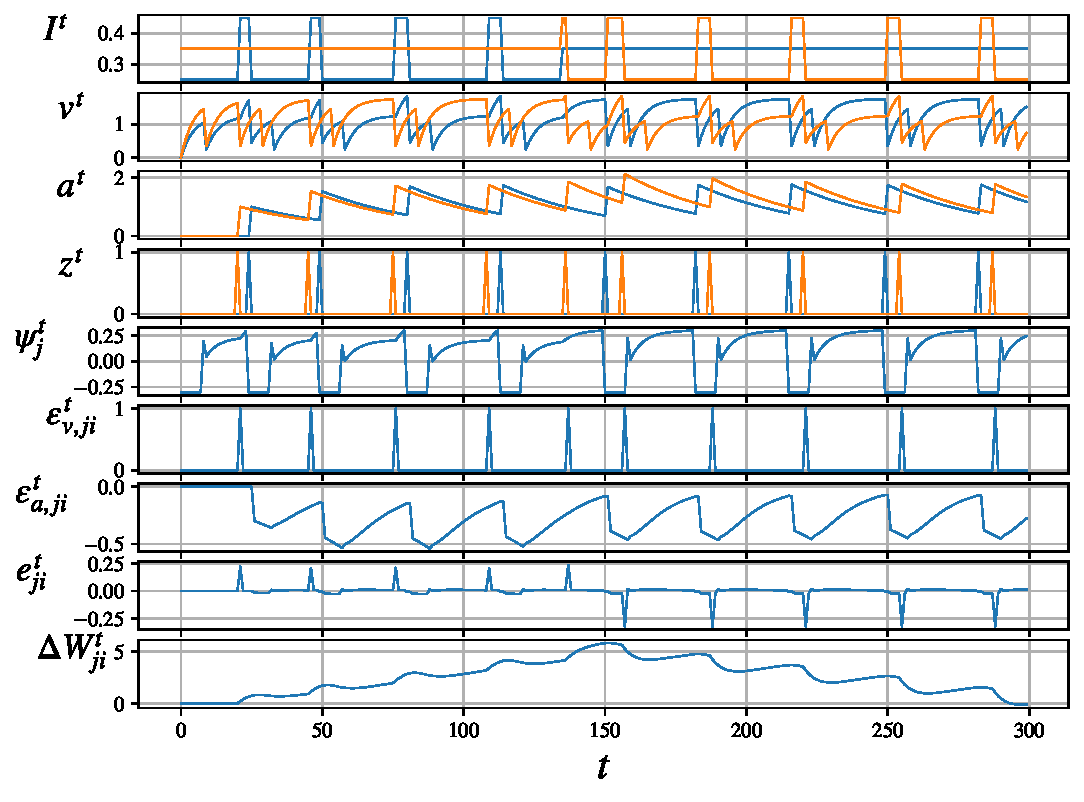
\includegraphics[width=\linewidth]{gfx/stdpalif}
	            \caption{A single-synapse demonstration of the STDP-ALIF.}
	            \label{fig:stdpalif}
	        \end{figure}

		\subsubsection{Izhikevich neuron}

			The standard system of equations of the Izhikevich neuron is described by
			\begin{align}
			v' &= 0.04v^2 + 5v + 140 - u + I\\
			a' &= 0.004v - 0.02a,
			\end{align}
			where $v'$ and $a'$ are the values of the activation value $v$ and recovery variable $a$ at the next time point, and $I$ is the current input to the neuron.
			Following \citet{traub2020learning}, the activation reset and refractory period are built into this system of equations by replacing $v$ and $a$ by respectively:
			\begin{align}
			\tilde{v}^t_{rj} &= v^t_{rj} - \left(v^t_{rj} + 65\right)z^t_{rj}\\
			\tilde{a}^t_{rj} &= a^t_{rj} + 2z^t_{rj},
			\end{align}
			such that when a spike event occurs (\ie, $z^t_{rj} = 1$), the activation value is reset to its baseline value of $-65$, and the recovery variable increases by 2.
			We describe this ``self-resetting'' Izhikevich neuron in the context of multi-layer e-prop as follows:
			\begin{align}
			v^{t+1}_{rj} &= \tilde{v}^t_{rj} + 0.04\left(\tilde{v}^t_{rj}\right)^2 + 5\tilde{v}^t_{rj} + 140 - \tilde{u}^t_{rj} + I^t_{rj}\\
			u^{t+1}_{rj} &= \tilde{u}^t_{rj} + 0.004\tilde{v}^t_{rj}-0.02\tilde{u}^t_{rj}.
			\end{align}
			The partial derivatives of the hidden state $\mathbf{h}^t_{rj}$ can then be computed:
			\begin{align}
			\frac{\partial v^{t+1}_{rj}}{\partial v^t_{rj}} &= \left(1-z^t_{rj}\right)\left(6+0.08v^t_{rj}\right)\\
			\frac{\partial a^{t+1}_{rj}}{\partial v^t_{rj}} &= -1\\
			\frac{\partial v^{t+1}_{rj}}{\partial a^t_{rj}} &= 0.004\left(1-z^t_{rj}\right)\\
			\frac{\partial a^{t+1}_{rj}}{\partial a^t_{rj}} &= 0.98.
			\end{align}

			Using these values, we compute the new eligibility trace:
	        \begin{align}
	        \mathbf{\epsilon}^{t+1}_{rji} &= \frac{\partial\mathbf{h}^{t+1}_{rj}}{\partial\mathbf{h}^t_{rj}}\cdot\mathbf{\epsilon}^t_{rji} + \frac{\partial\mathbf{h}^{t+1}_{rj}}{\partial W_{rji}}\\
	        &= \begin{pmatrix}\left(1-z^t_{rj}\right)\left(6+0.08v^t_{rj}\right)\epsilon^t_{rji, v} -\epsilon^t_{rji, a} + z_{ri}^{t-1}\\
	        0.004\left(1-z^t_{rj}\right)\epsilon^t_{rji, v} + 0.98\epsilon^t_{rji, a}
	        \end{pmatrix}\label{eq:ml_izhikevich_evector}
	        \end{align}
	        As in \citet{traub2020learning}, the pseudo-derivative is defined as
	        \begin{equation}
	        \psi^t_{rj} = \gamma\ \exp\left(\frac{\min\left(v^t_{rj}, 30\right) - 30}{30}\right),
	        \end{equation}
	        such that
	        \begin{equation}
	        \begin{pmatrix}\frac{\partial z^t_{rj}}{\partial v^t_{rj}}\\\frac{\partial z^t_{rj}}{\partial u^t_{rj}}\end{pmatrix}
	        = \begin{pmatrix}\psi^t_{rj}\\0\end{pmatrix}
	        \end{equation}
	        and therefore only $\epsilon^t_{rji, v}$ is used in computing the eligibility trace:
	        \begin{align}
	        e^t_{rji} &= \left(\psi^t_{rj}\ 0\right)\begin{pmatrix}\epsilon^t_{rji, v}\\\epsilon^t_{rji, a}\end{pmatrix} \\
	        &= \psi^t_{rj}\epsilon^t_{rji, v}.
	        \end{align}

	    However, when inserting these equations in a single-synapse demo, the eligibility vector assumes extremely high or low values (see Figure \ref{fig:demo_izh}).
	    This suggests that the Izhikevich neuron does not fit the e-prop framework well.
	    In this report, this is corrected by clipping the value of $\epsilon^t_{ji,v}$ to $\left[-3, 3\right]$ and $\epsilon^t_{ji,a}$ to $\left[-0.005, 0.005\right]$.
	    This correction yields the desired STDP behavior (see Figure \ref{fig:demo_izh_corrected}).

        \begin{figure}[ht]
            \centering
            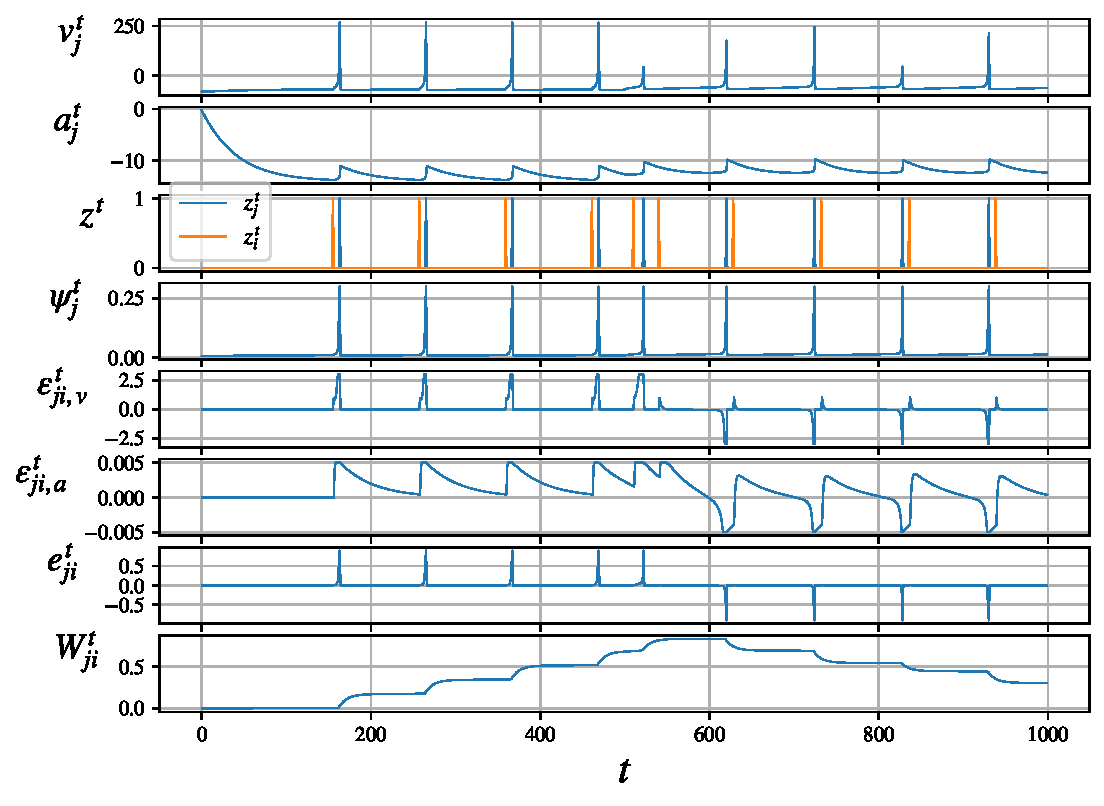
\includegraphics[width=\linewidth]{gfx/demo_izh_corrected}
            \caption{A single-synapse demo of the corrected Izhikevich neuron.}
            \label{fig:demo_izh_corrected}
        \end{figure}


\section{Regularization}

	Firing rate regularization and L2 regularization are applied to improve the stability of the learning process and the generalizability of the resulting model.
	These two regularization methods are motivated by biological plausibility, ease of implementation in the e-prop framework, and improved empirical performance.

	\subsection{Firing rate regularization}
		A firing rate regularization term is added to individually control the spike frequencies of the neurons.
		Since spikes in a neuromorphic architecture cost energy, the practical motivation for this regularization term is that it increases the energy efficiency of the model.
		The biological motivation is that the firing rate of biological neurons is also under homeostatic control \citep{erickson2006activity}.

		Firing rate is implemented by adding a regularization term $E_\text{reg}$ to the loss function that penalizes neurons that have a firing rate that is too low or too high:
		\begin{equation}
			E_\text{reg} = \frac{1}{2}\sum_j\left(f^\text{target} - f^{\text{av}, t}_{rj}\right)^2,
		\end{equation}
		where $f^\text{target}$ is a target firing rate of \SI{10}{\Hz}, and
		\begin{equation}
		f^{\text{av},t}_{rj} = \frac{1}{t} z^{\text{total},t}_{rj}
		\end{equation}
		is the running average spike frequency, where $z^{\text{total},t}$ accumulates spikes emitted by neuron $j$ in layer $r$ up to (and including) time step $t$.
		Note that $z^{\text{total},0} = 0$, \ie, the accumulation resets at every new training sample.
		By implementing this sum as a hidden variable, e-prop remains an online training algorithm when firing rate regularization is implemented.

		To insert the regularization term into the e-prop framework, we compute the weight update that regularizes the firing rate toward $f^\text{target}$ through gradient descent, similarly to the main e-prop weight update (Equation \ref{eq:eprop_grd}):
		\begin{equation}
		\frac{\partial E_\text{reg}}{\partial z_{rj}^t} = \left(f^\text{target} - f^{\text{av}, t}_{rj}\right).
		\end{equation}
		Note that this regularization loss differs from the firing rate regularization in \citet{bellec2020solution}, in which the firing rate is calculated in an offline fashion, by retroactively computing the average firing rate based on all spikes instead of only accumulated spikes.
		Note also that in \citet{bellec2020solution}, $\frac{\partial E_\text{reg}}{\partial z_{rj}^t}$ is multiplied with the eligibility trace $e^t_{rji}$, as in Equation \ref{eq:eprop_grd} to obtain the weight update, whereas in this report, the eligibility trace is omitted, resulting in a number of benefits:
		\begin{enumerate}
			\item It allows silent neurons that have infrequently spiking afferent neurons to more easily increase their firing rate, because their low afferent eligibility traces no longer nullifies the regularization gradient, and thereby results in a better empirical learning performance;
			\item It is more efficient in emulations on von Neumann machines, because the element-wise multiplication of $\frac{\partial E_\text{reg}}{\partial z_{rj}^t}$ and the eligibility trace is a relatively large computation on the order $\Theta\!\left(n^2\right)$ that no longer needs to be computed.
			\item It is more intuitive, as only the gradient of the firing rate is used to compute the weight update.
		\end{enumerate}
		We apply the weight update $\Delta W_{rji}$ of the regularization gradient using
		\begin{equation}
		\Delta_\text{reg} W_{rji} = -\eta\ c_\text{reg}\sum_t\left(f^\text{target} - f^{\text{av}, t}_{rj}\right).
		\end{equation}
		Note that the regularization gradients can be combined and accumulated over time on the same synaptic variable as the normal gradients, facilitating practical implementation of the learning procedure in both software emulations and neuromorphic embeddings:
		\begin{equation}
		\Delta W_{rji} = -\eta\ \sum_t\left(c_\text{reg}\left(f^\text{target} - f^{\text{av}, t}_{rj}\right) + L^t_{rj}\cdot\bar{e}^t_{rji}\right).
		\end{equation}

	\subsection{L2 regularization}
		To regularize weights around 0, a small fraction (parametrized by $c_\text{L2}$) of the value of the weight is added to its gradient value at every weight update:
		\begin{equation}
		\Delta_\text{L2} W_{rji} = -\eta\ c_\text{L2} \cdot W_{rji},
		\end{equation}
		which can be added to the full weight update as an extra term:
		\begin{equation}
		\Delta W_{rji} = -\eta\left(c_\text{L2} \cdot W_{rji} + \sum_t\left(c_\text{reg}\left(f^\text{target} - f^{\text{av}, t}_{rj}\right) + L^t_{rj}\cdot\bar{e}^t_{rji}\right)\right).
		\end{equation}
		The statistical motivation for this extra regularization term is that by softly restricting the weights, the network is less likely to overfit on the training data.

		The biological motivation is that biological synapses are regularized by a multiplicative factor to decrease the strength of individual synapses to the same proportion \citep{turrigiano2000hebb}, likely counteracting the run-away effects that the positive feedback of STDP naturally induces \citep{siddoway2014molecular}.
		Moreover, there are natural bounds of the strength of a biological synapse, measured by the amplitude of the postsynaptic potential, because the number of neurotransmitter vesicles and release sites is physically limited \citep{del1954quantal}.
		These natural limits are approximately \SI{0.4}{\mV} to \SI{20}{\mV} \citep{diaz2006target}.


% \section{Bidirectional network}
% 	\begin{tcolorbox}[colback=orange]
% 	- I/A
% 	- What, why, how?

% 	\end{tcolorbox}

\section{Optimizer}\label{sec:adam}

	For simplicity, in this report weight updates are described using stochastic gradient descent:
	\begin{equation}
		\Delta W_{rji} = -\eta \sum_t L^t_{rj}\cdot\bar{e}^t_{rji}.
	\end{equation}
	However, the results described in Chapter \ref{ch:results} are obtained using Adam (or Adaptive Moment Estimation) \citep{kingma2014adam}.
	This optimization method tracks running averages of the gradient and its second moment (resp. $M_{rji}$ and $V_{rji}$), and fits the local and online constraints of e-prop, because the running averages are tracked per individual synapse.
	The Adam weight update in the context of multi-layer e-prop is given by:
	\begin{align}
	M_{rji}^{(i+1)} &= \beta_1 M_{rji}^{(i)} + \left(1 - \beta_1\right)G^{(i)}_{rji} \\
	V_{rji}^{(i+1)} &= \beta_2 V_{rji}^{(i)} + \left(1 - \beta_2\right)\left(G^{(i)}_{rji}\right)^2 \\
	\widehat{M}_{rji} &= \frac{M_{rji}^{(i+1)}}{1 - \beta_1^{i+1}} \\
	\widehat{V}_{rji} &= \frac{V_{rji}^{(i+1)}}{1 - \beta_2^{i+1}} \\
	\Delta W_{rji}^{(i+1)} &= -\eta \frac{\widehat{M}_{rji}}{\sqrt{\widehat{V}_{rji}} + 10^{-5}},
	\end{align}
	where $G^{(i)}$ is the estimated gradient $\sum_t L^t_{rj}\cdot\bar{e}^t_{rji}$ at weight update $i$, and $\beta_1=0.9$ and $\beta_2=0.999$ are the forgetting factors for the gradient and its second moment, respectively.
	The firing rate and L2 regularization terms are omitted here for clarity.
	Note that the forgetting factors are not indexed, but raised to the power of $i+1$, in computing the bias-corrected estimates $\widehat{M}_{rji}$ and $\widehat{V}_{rji}$.
	Note also that minibatches of size 32 are used to more accurately estimate the gradient and enable a stabler descent in the error landscape.
	The value of $G^{(i)}_{rji}$ is computed as the mean over the minibatch.

	Note that the learning rate is linearly ramped up from 0 to $\eta$ during the first epoch, such that the initial minibatches are used to aggregate good initial momentum buffers, as the variance is higher when fewer minibatches are processed.
	This ``warming up'' of the learning rate is a variance reduction technique that has shown beneficial results in training other models \citep{liu2019variance}.
	Empirical observations on the resulting learning curves (see Chapter \ref{ch:results}) suggest that this procedure does not obstruct a rapid initial decrease of the loss function.

%************************************************
\chapter{Results}\label{ch:results}
%************************************************
In this chapter, the learning performance and regularization behavior of the ALIF, STDP-ALIF, and Izhikevich neurons are compared.
Then, the effect of stacking multiple recurrent layers on the learning performance and speed is examined.
Figure \ref{fig:inoutpair} shows a typical classification result of a full validation sentence.

	\begin{figure}[ht]
	    \myfloatalign
	    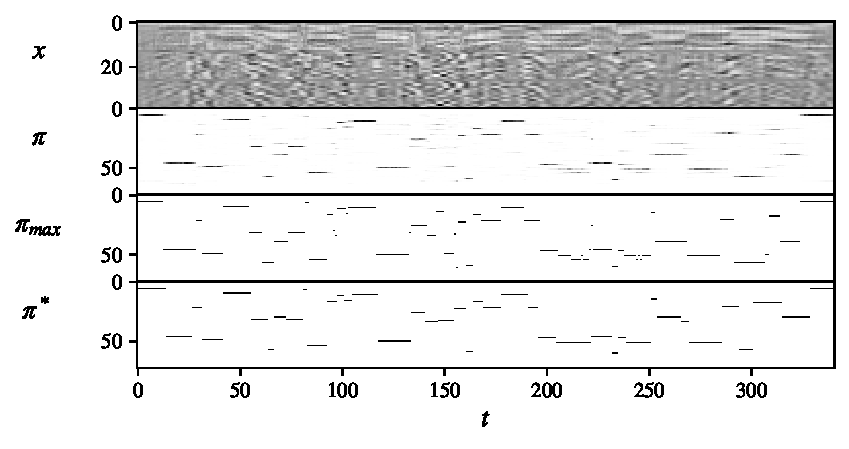
\includegraphics[width=\linewidth]{gfx/InOutPair}
	    \caption[Input-output-target example.]{An example validation result using a trained ALIF model. The top row shows the standardized MFCC frames of a sentence changing over time. The second row shows the probability distributions of the frame-wise outputs of the model. The third row is the most likely phone. The last layer shows the target phones.}
	    \label{fig:inoutpair}
	  \end{figure}

\section{Comparing neuron models}
	\paragraph{Accuracy}
		The main outcome of the neuron model comparison is that in these results, the Izhikevich neuron type performs poorly compared to the ALIF and STDP-ALIF neuron models, which reach a similar classification performance.
		In Figure \ref{fig:percwrong} the Izhikevich neuron reaches a misclassification rate of 94.2\% on the test set, which is only slightly better than constantly guessing the most frequent class.
		The ALIF neuron reaches a test misclassification rate of 50\% in relatively few iterations, and the STDP-ALIF stably reaches 50\%, and likely lower if training was continued for longer.
		Note that the test performance was obtained on the model with the best validation accuracy.

		Figure \ref{fig:crossentropy} illustrates the decrease of the cross-entropy score, which for the ALIF and STDP-ALIF neurons is comparable to that of the misclassification rate.
		The cross-entropy of the Izhikevich neuron continues to decrease while its classification accuracy stalls, suggesting that it trains its bias toward more frequent phone classes rather than learning a relationship between input MFCCs and classes.

		\begin{figure}[bth]
		    \myfloatalign
		    \subfloat[Percentage of samples wrongly classified.]
		    {\label{fig:percwrong}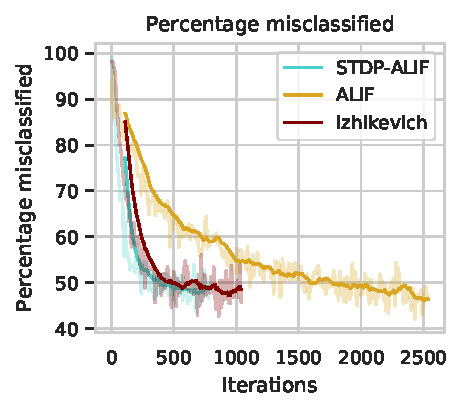
\includegraphics[height=5cm, keepaspectratio]{gfx/percwrong}} \quad
		    \subfloat[Cross-entropy loss (log-scaled).]
		    {\label{fig:crossentropy}%
		        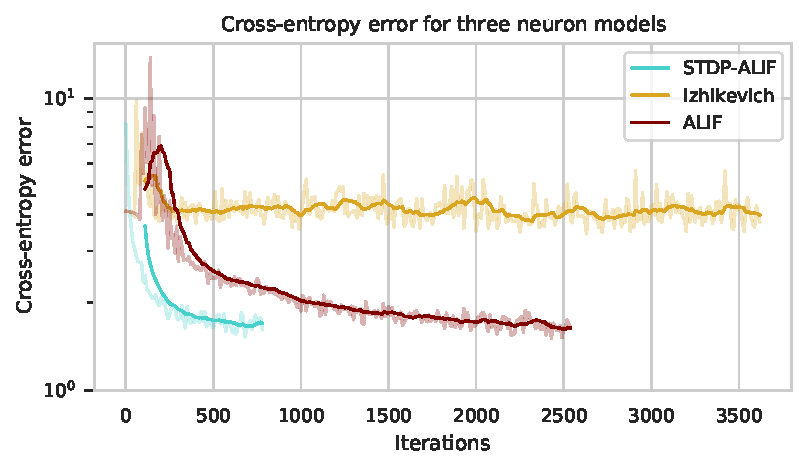
\includegraphics[height=5cm, keepaspectratio]{gfx/crossentropy}}
		    \caption[Classification performance for each of the three neuron models in a single-layer e-prop model.]{Classification performance on the validation data for each of the three neuron models in a single-layer e-prop model. The opaque lines indicate the running average of the real validation scores indicated by the transparent lines. The star symbols indicate the performances on the test set, with a misclassification rate of 92.4\% for the Izhikevich neuron, 50.3\% for the ALIF neuron, and 50\% for the STDP-ALIF neuron type.}\label{fig:sl-acc}
		\end{figure}

% testscores = {
% 	'ALIF': {1: (50.3, 1.772), 2: (64.5, 2.558), 3: (74.1, 3.345)},
% 	'STDP-ALIF': {1: (50.0, 1.751), 2: (65.3, 2.643), 3: (88.3, 4.779)},
% 	'Izhikevich': {1: (94.2, 6.794), 2: (88.2, 4.259), 3: (88.5, 4.161)}
% }

	\paragraph{Firing rate}
		Figure \ref{fig:freqs} illustrates the effect of the firing regularization term.
		It can be observed that the ALIF and STDP-ALIF neuron models are able to quickly change their mean spiking frequencies to the desired target frequency of \SI{10}{\Hz}, but the Izhikevich neuron increases past this rate to a spiking frequency of approximately \SI{18}{\Hz}.

		Figure \ref{fig:regerr} illustrates the decrease of the regularization error.
		The ALIF neuron appears to slightly better adapt to the regularization term.
		The Izhikevich neuron, again, underperforms significantly.
		\begin{figure}[bth]
		    \myfloatalign
		    \subfloat[Mean spiking frequency.]
		    {\label{fig:freqs}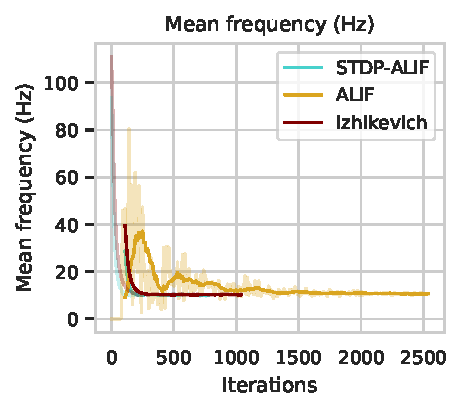
\includegraphics[height=5cm, keepaspectratio]{gfx/hz}} \quad
		    \subfloat[Regularization error.]
		    {\label{fig:regerr}%
		        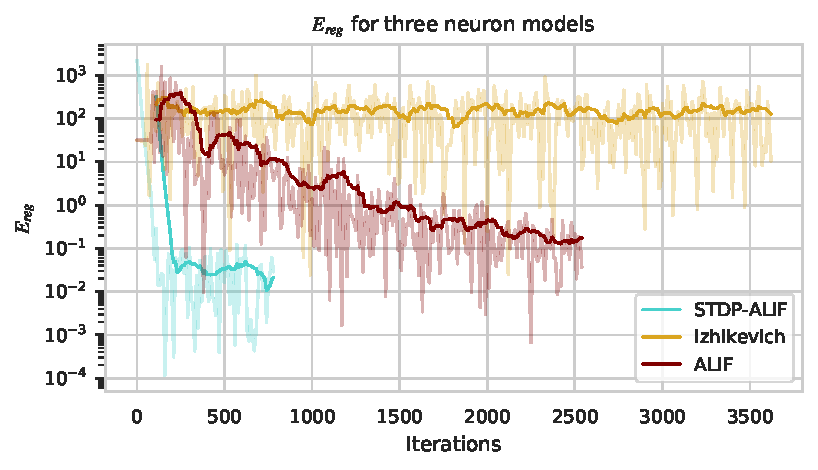
\includegraphics[height=5cm, keepaspectratio]{gfx/regerr}}
		    \caption[Effect of firing rate regularization for each of the three neuron models.]{Effect of firing rate regularization on the validation data for each of the three neuron models.}\label{fig:sl-reg}
		\end{figure}

\section{Comparing network depth}
The comparison between the network depth in Figures \ref{fig:ml-pwrong-alif}--\ref{fig:ml-pwrong-izh} suggests that single-layer e-prop networks train considerably more efficiently and accurately than multi-layer e-prop networks.
This holds for all tested neuron types.
The cross-entropy error, spiking frequency, and regularization error are also better for single-layer networks (see Figure \ref{fig:ml-otherresults}).

\begin{figure}[bth]
    \myfloatalign
    \subfloat[ALIF model.]
    {\label{fig:ml-pwrong-alif}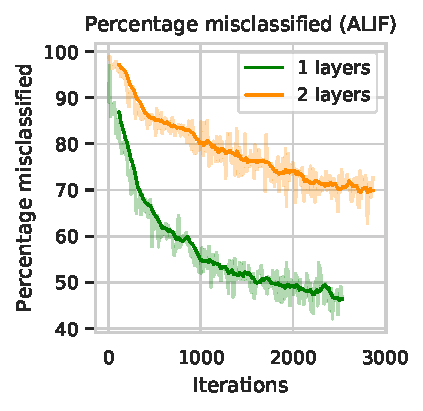
\includegraphics[height=5cm, keepaspectratio]{gfx/ml-percwrong-ALIF}} \quad
    \subfloat[STDP-ALIF model.]
    {\label{fig:ml-pwrong-stdpalif}%
        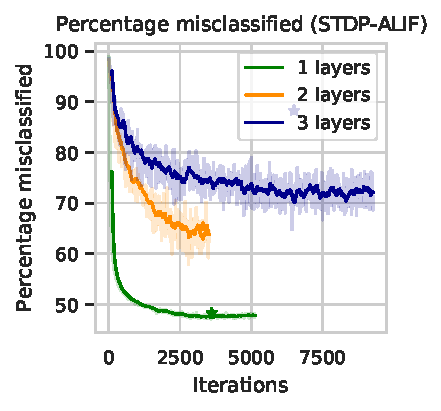
\includegraphics[height=5cm, keepaspectratio]{gfx/ml-percwrong-STDP-ALIF}} \\
    \subfloat[Izhikevich model.]
    {\label{fig:ml-pwrong-izh}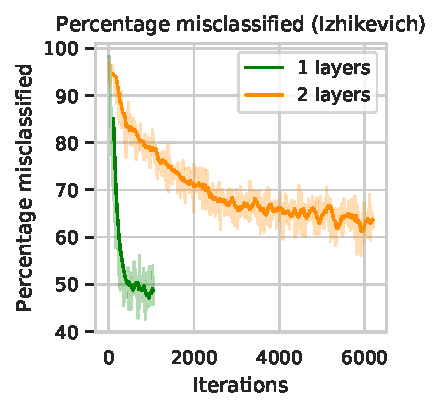
\includegraphics[height=5cm, keepaspectratio]{gfx/ml-percwrong-Izhikevich}}
    \caption[Single- and multi-layer accuracy comparison]{Accuracy comparison on the validation data between single- and multi-layer e-prop models.}\label{fig:ml-percwrong}
\end{figure}

%************************************************
\chapter{Discussion}\label{ch:discussion}
%************************************************

\paragraph{Interpretation of results}






%************************************************
\chapter{Conclusion}\label{ch:conclusion}
%************************************************

In this report, the e-prop framework was applied on the TIMIT phone classification task, meeting the objectives listed in Chapter \ref{ch:introduction}.

First, the performance of the ALIF neuron was reproduced using the explicit e-prop equations.
Next, the STDP-LIF neuron was modified to STDP-ALIF, and experimentally verified to perform competitively with ALIF.
Also, the Izhikevich neuron, which also shows STDP behavior, was shown to be unstable and performing worse than the ALIF and STDP-ALIF neurons.
This suggests that STDP does not provide an adequate neuron model by itself, but that \eg spike frequency adaptation also needs to be taken into account.

Finally, the effect of stacking multiple layers was also examined, and did not improve the learning performance in this task.

E-prop remains a framework that offers high potential for biologically plausible learning algorithms for SNNs, which can be particularly well-suited for replicating intelligent behavior in low-power neuromorphic hardware.



% ********************************************************************
% Backmatter
%*******************************************************
\appendix
%\renewcommand{\thechapter}{\alph{chapter}}
\cleardoublepage
%************************************************
\chapter{Appendix}\label{ch:appendix}
%************************************************


%********************************************************************
% Other Stuff in the Back
%*******************************************************
\cleardoublepage%********************************************************************
% Bibliography
%*******************************************************
% work-around to have small caps also here in the headline
% https://tex.stackexchange.com/questions/188126/wrong-header-in-bibliography-classicthesis
% Thanks to Enrico Gregorio
\defbibheading{bibintoc}[\bibname]{%
  \phantomsection
  \manualmark
  \markboth{\spacedlowsmallcaps{#1}}{\spacedlowsmallcaps{#1}}%
  \addtocontents{toc}{\protect\vspace{\beforebibskip}}%
  \addcontentsline{toc}{chapter}{\tocEntry{#1}}%
  \chapter*{#1}%
}
\printbibliography[heading=bibintoc]

% Old version, will be removed later
% work-around to have small caps also here in the headline
%\manualmark
%\markboth{\spacedlowsmallcaps{\bibname}}{\spacedlowsmallcaps{\bibname}} % work-around to have small caps also
%\phantomsection
%\refstepcounter{dummy}
%\addtocontents{toc}{\protect\vspace{\beforebibskip}} % to have the bib a bit from the rest in the toc
%\addcontentsline{toc}{chapter}{\tocEntry{\bibname}}
%\label{app:bibliography}
%\printbibliography

% \cleardoublepage%*******************************************************
% Declaration
%*******************************************************
\pdfbookmark[0]{Declaration}{declaration}
\chapter*{Declaration}
\thispagestyle{empty}
Put your declaration here.
\bigskip

\noindent\textit{\myLocation, \myTime}

\smallskip

\begin{flushright}
    \begin{tabular}{m{5cm}}
        \\ \hline
        \centering\myName \\
    \end{tabular}
\end{flushright}

% \cleardoublepage\pagestyle{empty}

\hfill

\vfill


\pdfbookmark[0]{Colophon}{colophon}
\section*{Colophon}
This document was typeset using the typographical look-and-feel \texttt{classicthesis} developed by Andr\'e Miede and Ivo Pletikosić.
The style was inspired by Robert Bringhurst's seminal book on typography ``\emph{The Elements of Typographic Style}''.
\texttt{classicthesis} is available for both \LaTeX\ and \mLyX:
\begin{center}
\url{https://bitbucket.org/amiede/classicthesis/}
\end{center}
Happy users of \texttt{classicthesis} usually send a real postcard to the author, a collection of postcards received so far is featured here:
\begin{center}
\url{http://postcards.miede.de/}
\end{center}
Thank you very much for your feedback and contribution.

\bigskip

\noindent\finalVersionString

%Hermann Zapf's \emph{Palatino} and \emph{Euler} type faces (Type~1 PostScript fonts \emph{URW
%Palladio L} and \emph{FPL}) are used. The ``typewriter'' text is typeset in \emph{Bera Mono},
%originally developed by Bitstream, Inc. as ``Bitstream Vera''. (Type~1 PostScript fonts were made
%available by Malte Rosenau and
%Ulrich Dirr.)

%\paragraph{note:} The custom size of the textblock was calculated
%using the directions given by Mr. Bringhurst (pages 26--29 and
%175/176). 10~pt Palatino needs  133.21~pt for the string
%``abcdefghijklmnopqrstuvwxyz''. This yields a good line length between
%24--26~pc (288--312~pt). Using a ``\emph{double square textblock}''
%with a 1:2 ratio this results in a textblock of 312:624~pt (which
%includes the headline in this design). A good alternative would be the
%``\emph{golden section textblock}'' with a ratio of 1:1.62, here
%312:505.44~pt. For comparison, \texttt{DIV9} of the \texttt{typearea}
%package results in a line length of 389~pt (32.4~pc), which is by far
%too long. However, this information will only be of interest for
%hardcore pseudo-typographers like me.%
%
%To make your own calculations, use the following commands and look up
%the corresponding lengths in the book:
%\begin{verbatim}
%    \settowidth{\abcd}{abcdefghijklmnopqrstuvwxyz}
%    \the\abcd\ % prints the value of the length
%\end{verbatim}
%Please see the file \texttt{classicthesis.sty} for some precalculated
%values for Palatino and Minion.
%
%    \settowidth{\abcd}{abcdefghijklmnopqrstuvwxyz}
%    \the\abcd\ % prints the value of the length

% ************************************************************
\end{document}
% ********************************************************************


* RESULTS
  - Comparing single-layer and multilayer architecture. Some of the following. Explain and visualize!
    - Accuracy
    - Tradeoffs between network size and accuracy (not necessarily same hparams)
    - Time/manifold dynamics
    - Effects of parameter changes
    - Effects of weight freezes (also include only training output or not at all)
    - Energy
    - Robustness (initialization, data, and hparam).
    - Practicality (e.g. running cost in-sim or in-mat, AER options)

* DISCUSSION
  - Try link/explain results with existing research. Show knowledge of the field.
  - Advantages of e-prop RSNN
    - Computational cost of backprop vs BA.
  - Link to R-STDP with Traub fix -> section on biological plausibility and analogies. Three-factor Hebbian learning.
  - Neuromorphic computing applications for benefits (parallelization, energy cost).
  - Maybe: if manifolds of phones, then hypothesize on self-symbolizing (as in Hofstadter). Try to link my own hypotheses to scientific evidence. Keep it relevant to the rest of the paper.
  - Trend to bioplausibility -?-> artificial consciousness? Cite!
  - Future research (also ask Herbert)

* CONCLUSION
  - Powerful and engaging!
  - Short summary, key sentences from all previous. Logical connection to introduction.
  - Neuromorphic computing
  - Maybe: attempt to explain network interpretability. Subgraphs representing features.

* APPENDIX
  - Explain implementation, sweeping, and all details such that precise replication can be made.
  - Pseudocode


=================

[Direct proof]
<Indirect proof>
(Only assert)

TALKING POINTS I COULD USE:

* INTRODUCTION
  - Brain is different from deep ANNs <Bellec1>
  - RNNs superior for temporal dimension (Bellec1)
  - BPTT is implausible for neuromorphic (Bellec1)
  - Three-factor Hebbian learning in RSNN is competitive with BPTT [Bellec1]
  - E-prop better RSNN learning performance than previously known methods [Bellec1]
  -
